%%%%%%%%%%%%%%%%%%%%%%%%%%%%%%%%%%%%%%%%%%%%%%%%%%
%DIF LATEXDIFF DIFFERENCE FILE
%DIF DEL JASA - Round 1/Eng-vowel-norm.tex   Sun Nov 10 14:01:28 2024
%DIF ADD Eng-vowel-norm.tex                  Tue Nov 12 18:38:35 2024
%  JASA LaTeX Template File
%  To make articles using JASA.cls, Version 1.1
%  September 14, 2019
%%%%%%%%%%%%%%%%%%%%%%%%%%%%%%%%%%%%%%%%%%%%%%%%%%

%% Step 1:
%% Uncomment the style that you want to use:

%%%%%%% For Preprint
%% For manuscript, 12pt, one column style

\documentclass[preprint]{JASA}

%%%%% Preprint Options %%%%%
%% The track changes option allows you to mark changes
%% and will produce a list of changes, their line number
%% and page number at the end of the article.
%\documentclass[preprint,trackchanges]{JASA}


%% NumberedRefs is used for numbered bibliography and citations.
%% Default is Author-Year style.
%% \documentclass[preprint,NumberedRefs]{JASA}

%%%%%%% For Reprint
%% For appearance of finished article; 2 columns, 10 pt fonts

% \documentclass[reprint]{JASA}

%%%%% Reprint Options %%%%%

%% For testing to see if author has exceeded page length request, use 12pt option
%\documentclass[reprint,12pt]{JASA}


%% NumberedRefs is used for numbered bibliography and citations.
%% Default is Author-Year style.
% \documentclass[reprint,NumberedRefs]{JASA}

%% TurnOnLineNumbers
%% Make lines be numbered in reprint style:
% \documentclass[reprint,TurnOnLineNumbers]{JASA}

\usepackage{natbib}




% tightlist command for lists without linebreak
\providecommand{\tightlist}{%
  \setlength{\itemsep}{0pt}\setlength{\parskip}{0pt}}

% From pandoc table feature
\usepackage{longtable,booktabs,array}
\usepackage{calc} % for calculating minipage widths
% Correct order of tables after \paragraph or \subparagraph
\usepackage{etoolbox}
\makeatletter
\patchcmd\longtable{\par}{\if@noskipsec\mbox{}\fi\par}{}{}
\makeatother
% Allow footnotes in longtable head/foot
\IfFileExists{footnotehyper.sty}{\usepackage{footnotehyper}}{\usepackage{footnote}}
\makesavenoteenv{longtable}



\usepackage{tikz}
\usetikzlibrary{bayesnet}
% rotating must be loaded before tablefootnote
% \usepackage{rotating}
\usepackage{multirow}
\usepackage{colortbl}
\usepackage{tablefootnote}
\usepackage{amssymb}
\usepackage[caption=false]{subfig}
\usepackage{setspace}
%DIF 78a78-80
% For references to external document %DIF > 
\usepackage{xr} %DIF > 
\externaldocument{manuscript-with-SI} %DIF > 
%DIF -------

\usepackage{fontspec}

%% Special font for IPA
%% Make sure "Doulos SIL" is installed on your computer
%% For other typefaces supporting IPA symbols, see
%% https://en.wikipedia.org/wiki/International_Phonetic_Alphabet#Typefaces
\newfontfamily\ipa{Doulos SIL} % Font for IPA symbols
\DeclareTextFontCommand{\ipatext}{\ipa}

%%%         Section for CJK Characters                   %%%
%%%   You may want to uncomment the code below if        %%%
%%%   you're writing this document with CJK characters   %%%

%\usepackage{xeCJK}  % Uncomment for using CJK characters
%% Set main font for CJK characters
%% Make sure your system has the font set
%\setCJKmainfont[
%	BoldFont={HanWangHeiHeavy}  % Set font for CJK boldface
%    ]{標楷體}    % Set font for normal CJK
%% Some Traditional Chinese fonts: AR PL KaitiM Big5, PingFang TC, Noto Sans CJK TC
%\XeTeXlinebreaklocale "zh"
%\XeTeXlinebreakskip = 0pt plus 1pt

%% Added by Florian to make biblatex and its \refsection work since pandoc does not parse 
%% content within latex environments. \refsection in turn is required to allow authors
%% to have multiple separate bibliographies (here: one for main text and one for SI).
%%
%% For some reasons it does seem to be necessary to reload the bibpackage here since
%% ---at least for my system---adding the following to the YAML header instead does
%% not seem to work:
%%
%%    biblio-style: apa
%%    biblatexoptions: [backend=biber,maxbibnames=999,style=apa]
%% 
%% curiously removing the following from the YAML header:
%%
%%     citation_package: biblatex
%%
%% makes knitr (or pandoc?) revert back to the default bibtex treatment, which does 
%% not allow multiple bibliographies.
% \usepackage[backend=biber, maxbibnames=999, style=apa]{biblatex}
% \addbibresource{latex-stuff/library.bib}
% \newcommand{\brefsection}{\begin{refsection}}
% \newcommand{\erefsection}{\end{refsection}}

\newcommand{\changelocaltocdepth}[1]{%
  \addtocontents{toc}{\protect\setcounter{tocdepth}{#1}}%
  \setcounter{tocdepth}{#1}%
}
\setcounter{tocdepth}{-10}
\changelocaltocdepth{-10}
%DIF PREAMBLE EXTENSION ADDED BY LATEXDIFF
%DIF UNDERLINE PREAMBLE %DIF PREAMBLE
\RequirePackage[normalem]{ulem} %DIF PREAMBLE
\RequirePackage{color}\definecolor{RED}{rgb}{1,0,0}\definecolor{BLUE}{rgb}{0,0,1} %DIF PREAMBLE
\providecommand{\DIFadd}[1]{{\protect\color{blue}\uwave{#1}}} %DIF PREAMBLE
\providecommand{\DIFdel}[1]{{\protect\color{red}\sout{#1}}}                      %DIF PREAMBLE
%DIF SAFE PREAMBLE %DIF PREAMBLE
\providecommand{\DIFaddbegin}{} %DIF PREAMBLE
\providecommand{\DIFaddend}{} %DIF PREAMBLE
\providecommand{\DIFdelbegin}{} %DIF PREAMBLE
\providecommand{\DIFdelend}{} %DIF PREAMBLE
\providecommand{\DIFmodbegin}{} %DIF PREAMBLE
\providecommand{\DIFmodend}{} %DIF PREAMBLE
%DIF FLOATSAFE PREAMBLE %DIF PREAMBLE
\providecommand{\DIFaddFL}[1]{\DIFadd{#1}} %DIF PREAMBLE
\providecommand{\DIFdelFL}[1]{\DIFdel{#1}} %DIF PREAMBLE
\providecommand{\DIFaddbeginFL}{} %DIF PREAMBLE
\providecommand{\DIFaddendFL}{} %DIF PREAMBLE
\providecommand{\DIFdelbeginFL}{} %DIF PREAMBLE
\providecommand{\DIFdelendFL}{} %DIF PREAMBLE
%DIF END PREAMBLE EXTENSION ADDED BY LATEXDIFF

\begin{document}
%% the square bracket argument will send term to running head in
%% preprint, or running foot in reprint style.

\title[Comparing normalization against perception]{Comparing accounts of formant normalization against US English listeners' vowel perception}

% ie
%\title[JASA/Sample JASA Article]{Sample JASA Article}

%% repeat as needed

\author{Anna Persson}
% ie
%\affiliation{Department1,  University1, City, State ZipCode, Country}
\DIFdelbegin %DIFDELCMD < \affiliation{Swedish Language and Multilingualism, Stockholm University}
%DIFDELCMD < %%%
\DIFdelend \DIFaddbegin \affiliation{Swedish Language and Multilingualism, Stockholm University, Stockholm, SE-106 91, Sweden}
\DIFaddend %% for corresponding author
\email{anna.persson@su.se}
%% for additional information

\author{Santiago Barreda}
% ie
%\affiliation{Department1,  University1, City, State ZipCode, Country}
\affiliation{Linguistics, University of California, Davis}
%% for corresponding author

%% for additional information

\author{T. Florian Jaeger}
% ie
%\affiliation{Department1,  University1, City, State ZipCode, Country}
\affiliation{Brain and Cognitive Sciences, Data Science, University of Rochester}
%% for corresponding author

%% for additional information


% ie
% \author{Author Four}
% \email{author.four@university.edu}
% \thanks{Also at Another University, City, State ZipCode, Country.}

%% For preprint only,
%  optional, if you want want this message to appear in upper left corner of title page
\preprint{Persson, Barreda, \& Jaeger, JASA}

%ie
%\preprint{Author, JASA}

% optional, if desired:
%\date{\today}
\date{\today}

\begin{abstract}
% Put your abstract here. Abstracts are limited to 200 words for
% regular articles and 100 words for Letters to the Editor. Please no
% personal pronouns, also please do not use the words ``new'' and/or
% ``novel'' in the abstract. An article usually includes an abstract, a
% concise summary of the work covered at length in the main body of the
% article.
Human speech \DIFdelbegin \DIFdel{perception tends to achieve robustspeech recognition}\DIFdelend \DIFaddbegin \DIFadd{recognition tends to be robust}\DIFaddend , despite substantial cross-talker variability. Believed to be critical to this ability are auditory normalization mechanisms whereby listeners adapt to individual differences in vocal tract physiology\DIFdelbegin \DIFdel{in vowel perception}\DIFdelend . This study \DIFdelbegin \DIFdel{asks what types of computations are }\DIFdelend \DIFaddbegin \DIFadd{investigates the computations }\DIFaddend involved in such normalization. Two 8-way alternative forced-choice experiments assessed L1 listeners' categorizations across the entire US English vowel space---both for unaltered and for synthesized stimuli. Listeners' responses in these experiments were compared against the predictions of twenty influential normalization accounts that differ starkly in the inference and memory capacities they imply for speech perception. \DIFaddbegin \DIFadd{This includes variants of }\emph{\DIFadd{estimation-free}} \DIFadd{transformations into psycho-acoustic spaces, }\emph{\DIFadd{intrinsic}} \DIFadd{normalizations relative to concurrent acoustic properties, and }\emph{\DIFadd{extrinsic}} \DIFadd{normalizations relative to talker-specific statistics. }\DIFaddend Listeners' responses were best explained by \DIFdelbegin \emph{\DIFdel{extrinsic}} %DIFAUXCMD
\DIFdel{normalizationaccounts}\DIFdelend \DIFaddbegin \DIFadd{extrinsic normalization}\DIFaddend , suggesting that listeners learn and store distributional properties of talkers' speech. \DIFdelbegin \DIFdel{Of the extrinsic accounts, it was the }\DIFdelend \DIFaddbegin \DIFadd{Specifically, }\DIFaddend \emph{computationally \DIFdelbegin \DIFdel{least complex}\DIFdelend \DIFaddbegin \DIFadd{simple}\DIFaddend } \DIFdelbegin \DIFdel{variants that }\DIFdelend \DIFaddbegin \DIFadd{(single-parameter) extrinsic normalization }\DIFaddend best fit listeners' responses\DIFdelbegin \DIFdel{, using a single parameter. These findings have consequences for any research that aims to investigate the perceptual, social, and linguistic information of vowel productions. This includes research in }\DIFdelend \DIFaddbegin \DIFadd{. This simple extrinsic normalization also clearly outperformed Lobanov normalization---a computationally more complex account that remains popular in research on }\DIFaddend phonetics and phonology, sociolinguistics, \DIFaddbegin \DIFadd{typology, }\DIFaddend and language acquisition.
\DIFdelbegin \DIFdel{In these fields, it remains common to employ normalization accounts that the present study confirms to be inadequate models of human perception (e.g., Lobanov normalization).
}\DIFdelend \end{abstract}

%% pacs numbers not used

\maketitle

%  End of title page for Preprint option --------------------------------- %

%% See preprint.tex/.pdf or reprint.tex/.pdf for many examples


%  Body of the article
\setcounter{secnumdepth}{5}
\setcounter{page}{1}
\setcounter{section}{0}

\section{Introduction}\label{sec:intro}

One of the central challenges for speech perception originates in cross-talker variability: depending on the talker, the same acoustic signal can encode different sound categories \citep{allen2003, liberman1967, newman2001}. This results in ambiguity in the mapping from acoustics to words and meanings. Research has identified several mechanisms through which listeners resolve this ambiguity, ranging from early perceptual processes, to adaptation of phonetic categories, all the way to adjustments in post-linguistic decision processes \citep[for review, see][]{xie2023}. The present study focuses on the first type of mechanism, early auditory processes that transform and normalize the acoustic input into the perceptual cues that constitute the input to linguistic processing \citep[for reviews,][]{barreda2020, johnson-sjerps2021, mcmurray-jongman2011, stilp2020, weatherholtz-jaeger2016}. We seek to respond, in particular, to recent calls to put theories of adaptive speech perception to stronger tests \citep{baeseberk2018, schertz-clare2020, xie2023}.

Evidence for the presence of early normalization mechanisms comes from neuroimaging and neurophysiological studies \citep[e.g.,][]{oganian2023, skoe2021}\DIFdelbegin \DIFdel{. These studies have }\DIFdelend \DIFaddbegin \DIFadd{, as well as research on the peripheral auditory system suggesting automatic transformations of the acoustic signal into scale-invariant spectral patterns }\citep[e.g.,][]{patterson2014, smith2005}\DIFadd{. Neurophysiological studies have further }\DIFaddend decoded effects of talker identity from subcortical brain areas like the brain stem, and thus prior to the cortical regions believed to encode linguistic categories \citep[e.g.,][]{sjerps2019, tang2017}. This includes brain responses that lag the acoustic signal by as little as 20-50 msecs \citep{lee2009}, suggesting very fast and highly automatic processes. \DIFdelbegin \DIFdel{By removing talker-specific variability from the phonetic signal early , auditory normalization offers }\DIFdelend \DIFaddbegin \DIFadd{While this does not mean that }\emph{\DIFadd{only}} \DIFadd{talker-normalized auditory percepts are available to subsequent processing---there is now convincing evidence that subcategorical information can enter listeners' phonetic representations }\citep[e.g.,][]{hay2017, hay2019, johnson1999, mcgowan2015, walker-hay2011}\DIFadd{---it does suggest that normalized auditory percepts are available to subsequent processing. By removing (some) cross-talker variability early during auditory processing, normalization offers an }\DIFaddend elegant and effective \DIFdelbegin \DIFdel{solutions to cross-talker variability, that might }\DIFdelend \DIFaddbegin \DIFadd{solution that can }\DIFaddend reduce the need for more complex \DIFdelbegin \DIFdel{adaptation of individual phonetic categories }\DIFdelend \DIFaddbegin \DIFadd{adaptive processes }\DIFaddend further upstream \citep{apfelbaum-mcmurray2015, xie2023}.
\DIFdelbegin \footnote{\DIFdel{Normalization does not necessarily imply that }\emph{\DIFdel{only}} %DIFAUXCMD
\DIFdel{talker-normalized auditory percepts are available to subsequent processing. There is ample evidence that subcategorical information can enter listeners' representations of sound categories }%DIFDELCMD < \citep[e.g.,][]{hay2017, hay2019, johnson1999, mcgowan2015, walker-hay2011}%%%
\DIFdel{, in line with episodic }%DIFDELCMD < \citep{goldinger1996} %%%
\DIFdel{and exemplar theory of speech perception }%DIFDELCMD < \citep{johnson1997, sumner2011}%%%
\DIFdel{.}}
%DIFAUXCMD
\addtocounter{footnote}{-1}%DIFAUXCMD
\DIFdelend 

While it is relatively uncontroversial \emph{that} normalization contributes to robust speech perception, it is still unclear what types of computations this implicates. We address this question for the perception of vowels, which cross-linguistically relies on peaks in the distribution of spectral energy over acoustic frequencies (formants).\DIFaddbegin \footnote{\DIFadd{Some hypotheses hold that robust speech perception does not require normalization, and that research on normalization has over-estimated its effectiveness because studies tend to consider only a fraction of the phonetic information available to listeners }\citep[for review, see][]{strange-jenkins2012}\DIFadd{. For vowel recognition, for example, listeners might use cues other than just formants }\citep{hillenbrand2006, nearey-assmann1986}\DIFadd{, and/or might use information about the dynamic development of formant trajectories over the entire vowel rather than just point estimates of formants at the vowel center }\citep[e.g.,][]{shankweiler1978}\DIFadd{. We return to this in the general discussion but note that even studies who use much richer inputs have found that normalization provides a better fit to listeners' perception }\citep{richter2017}\DIFadd{.}} \DIFaddend Vowel perception has long been a focus in research on normalization \citetext{\citealp[e.g.,][]{bladon1984}; \citealp{fant1975}; \citealp{gerstman1968}; \citealp{johnson2020}; \citealp{joos1948}; \citealp{lobanov1971}; \citealp{miller1989}; \citealp{nearey1978}; \citealp{nordstrom-lindblom1975}; \citealp{syrdal-gopal1986}; \citealp{traunmuller1981}; \citealp{watt-fabricius2002}; \citealp{zahorian-jagharghi1991}; \citealp[for review, see][]{barreda2020}}, with some reviews citing over 100 competing proposals \citep{carpenter-govindarajan1993}. Importantly, these accounts differ in the types and complexity of computations they assume to take place during normalization.
\DIFaddbegin 

\DIFaddend On the lower end of computational complexity, \DIFdelbegin \DIFdel{comparatively simple static transformations of the acoustic signal might suffice to achieve invariance in the mapping from cues to phonetic categories}\DIFdelend \DIFaddbegin \emph{\DIFadd{estimation-free}} \DIFadd{psycho-acoustic transformations involve zero degrees of freedom that listeners would need to estimate from the acoustic input}\DIFaddend . For example, there is evidence that a transformation of acoustic frequencies (measured in Hz) into the psycho-acoustic \DIFdelbegin \DIFdel{Mel-space }\DIFdelend \DIFaddbegin \DIFadd{Bark-space }\DIFaddend better describes how listeners perceive differences \DIFdelbegin \DIFdel{in the frequency of sine tones }%DIFDELCMD < \citetext{\citealp[e.g.,][]{fastl-zwicker2007}; \citealp{stevens-volkmann1940}; \citealp[for a critique, see][]{greenwood1997}; \citealp{siegel1965}}%%%
\DIFdelend \DIFaddbegin \DIFadd{along the frequency spectrum }\citep[in terms of critical bands, e.g.,][]{traunmuller1990, zwicker1957, zwicker1961, zwicker-terhardt1980}\DIFaddend . It is thus possible that cross-talker variability in vowel pronunciations is \DIFdelbegin \DIFdel{effectively }\DIFdelend reduced when formants are represented in \DIFdelbegin \DIFdel{Mel}\DIFdelend \DIFaddbegin \DIFadd{Bark}\DIFaddend , rather than Hz. Similar arguments have been made about other psycho-acoustic transformations \DIFdelbegin %DIFDELCMD < \citetext{\citealp[e.g., Bark,][]{traunmuller1990}; \citealp[ERB,][]{glasberg-moore1990}; \citealp[or semitones,][]{fant2002}}%%%
\DIFdel{. Most of these accounts }\DIFdelend \DIFaddbegin \citetext{\citealp[e.g., ERB,][]{glasberg-moore1990}; \citealp[Mel,][]{stevens-volkmann1940}; \citealp[or semitones,][]{fant2002}} \DIFadd{most of which }\DIFaddend share that they log-transform acoustic frequencies---in line with neurophysiological evidence that the auditory representations in the brain seem to follow a roughly logarithmic organization, so that auditory perception is (up to a point) more sensitive to differences between lower frequencies than to the same difference between higher frequencies \citetext{\citealp[e.g.,][]{merzenich1975}; \citealp[for review, see][]{saenz-langers2014}}. \DIFdelbegin \DIFdel{If such static }\DIFdelend \DIFaddbegin \DIFadd{While each of these transformations was developed with different applications in mind }\citetext{\citealp[e.g., ERB and Bark to explain frequency selectivity,][]{glasberg-moore1990}; \citealp[or semitones for the perception of musical pitch,][]{balzano1982}}\DIFadd{, }\DIFaddend psycho-acoustic transformations \DIFdelbegin \DIFdel{are sufficient for formant normalization}\DIFdelend \DIFaddbegin \DIFadd{might suffice for effective formant normalization. If so}\DIFaddend , this would offer a particularly parsimonious account of vowel perception as listeners would not have to infer talker-specific properties.

The parsimony of psycho-acoustic transformations contrasts with the majority of accounts for vowel normalization, which introduce additional computations. This includes accounts that normalize formants relative to other information that is available at the same point in the acoustic signal \citep[intrinsic normalization, e.g.,][]{miller1989, peterson1961, syrdal-gopal1986}. For example, according to one proposal, listeners normalize vowel formants by the vowel's fundamental frequency or other formants estimated at the same point in time \citep{syrdal-gopal1986}. To the extent that the fundamental frequency is correlated with the talkers' vocal tract size \citep[for review, see][]{vorperian-kent2007}, this allows the removal of physiologically-conditioned cross-talker variability in formant realizations. While such intrinsic accounts arguably entail more computational complexity than \DIFdelbegin \DIFdel{static }\DIFdelend \DIFaddbegin \DIFadd{estimation-free }\DIFaddend transformations, they do not require that listeners \emph{maintain} talker-specific estimates over time. This distinguishes intrinsic from extrinsic accounts, which introduce additional computational complexity.

According to extrinsic accounts, normalization mechanisms infer and store estimates of talker-specific properties that then are used to normalize subsequent speech from that talker \DIFdelbegin %DIFDELCMD < \citetext{\citealp{gerstman1968}; \citealp{lobanov1971}; \citealp{nearey1978}; \citealp{nordstrom-lindblom1975}; \citealp{watt-fabricius2002}; \citealp[for review, see also][]{weatherholtz-jaeger2016}}%%%
\DIFdelend \DIFaddbegin \citetext{\citealp{gerstman1968}; \citealp{lobanov1971}; \citealp{nearey1978}; \citealp{nordstrom-lindblom1975}; \citealp{watt-fabricius2002}; \citealp[for review, see][]{weatherholtz-jaeger2016}}\DIFaddend . At the upper end of computational complexity, some accounts hold that listeners continuously infer and maintain both talker-specific means for each formant and talker-specific estimates of each formant's variability \citep{gerstman1968, lobanov1971}. These estimates are then used to normalize formants, e.g., by centering and standardizing them \citep[essentially z-scoring formants,][]{lobanov1971}, removing cross-talker variability in the distribution of formant values. There are, however, more parsimonious extrinsic accounts that require inference and maintenance of fewer talker-specific properties. The most parsimonious of these is Nearey's \emph{uniform scaling} account, which assumes that listeners infer and maintain a single talker-specific parameter. This parameter (\(\Psi\)) can be thought of as capturing the effects of the \DIFdelbegin \DIFdel{talkers'}\DIFdelend \DIFaddbegin \DIFadd{talker's }\DIFaddend vocal tract length on the spectral scaling applied to the formant pattern produced by a talker \citep{nearey1978}.\footnote{Under uniform scaling accounts, listeners essentially `slide' the center of their category representations (e.g, the `template' of vowel categories for a given dialect) along a single line in formant space, with \(\Psi\) determining the target of this sliding. Later extensions of this account maintain its memory parsimony but increased its inference complexity by allowing both intrinsic (the current F0) and extrinsic information (the talker's single mean of log-transformed formants) to influence the inference of \(\Psi\) \citep{nearey-assmann2007}.\DIFdelbegin \DIFdel{We return to this extension in the general discussion.}\DIFdelend } Uniform scaling deserves particular mention here as it is arguably one of the most developed normalization accounts, and rooted in principled considerations about the physics of sound and the evolution of auditory systems \citep[for review, see][]{barreda2020}.

In summary, hypotheses about the computations implied by formant normalization differ in the flexibility they afford as well as the inference and memory complexity they entail. Considerations about the complexity of inferences---essentially the number of parameters that listeners are assumed to estimate at any given moment in time---arguably gain in importance in light of the speed at which normalization seems to unfold. In the present study, we thus ask whether computationally simple accounts are sufficient to explain human vowel perception.



\begin{figure}

{\centering \includegraphics[width=0.95\linewidth]{../../figures/knitted/two-talkers} 

}

\caption{Illustration of how height, which is positively correlated with vocal tract size, affects vowels' F1 and F2, and how normalization can partially remove this effect. Shown here are realizations of \DIFdelbeginFL \DIFdelFL{all 8 }\DIFdelendFL \DIFaddbeginFL \DIFaddFL{eight }\DIFaddendFL monophthong vowels of US English by a short (cyan) and a tall native talker (red). \textbf{Panel A:} In the acoustic space, prior to any normalization (Hz). \textbf{Panel B:} After uniform scaling \citep{nearey1978}. \textbf{Panel C:} After Lobanov normalization \citep{lobanov1971}. The present study compares \DIFdelbeginFL \DIFdelFL{three of }\DIFdelendFL these \DIFaddbeginFL \DIFaddFL{three }\DIFaddendFL accounts, along with 17 other normalization accounts. \DIFaddbeginFL \DIFaddFL{Here and throughout the paper, panel captions indicate the phonetic space in which normalization takes place in parenthesis. Note that this is not necessarily identical to the units of F1 and F2 }\emph{\DIFaddFL{after}} \DIFaddFL{normalization (e.g., Lovabov normalization results in scale-free z-scores along the formant axes).}\DIFaddendFL }\label{fig:two-talkers}
\end{figure}

While previous research has compared normalization accounts across languages, most of this work has evaluated proposals in terms of how well the normalized phonetic space supports the separability of vowel categories \citep{adank2004, carpenter-govindarajan1993, cole2010, escudero-bion2007, johnson-sjerps2021, syrdal1985}. This approach is illustrated in Figure \ref{fig:two-talkers}. These studies have found that computationally more complex accounts---which also afford more flexibility---tend to achieve higher category separability and higher categorization accuracy \citep[for review, see][]{persson-jaeger2023}. This includes Lobanov normalization, which continues to be highly influential in, for example, variationist and sociolinguistic research because of its effectiveness in removing cross-talker variability \citep[for a critique, see][]{barreda2021}. It is, however, by no means clear that human speech perception employs the same computations that achieve the best category separability or accuracy \citep[see also discussion in][]{barreda2021, nearey-assmann2007}.

A substantially smaller body of research has addressed this question by comparing normalization accounts against \emph{listeners' perception} \citetext{\citealp{barreda-nearey2012}; \citealp{barreda2021}; \citealp{nearey1989}; \citealp{richter2017}; \citealp[for a review, see][]{whalen2016}}. Interestingly, these works seem to suggest that computationally simpler accounts might provide a better fit against human speech perception than the influential Lobanov model \citep{barreda2021, richter2017}. For example, \citet{barreda2021} compared the predictions of uniform scaling and Lobanov normalization against listeners' categorization responses in a forced-choice categorization task over parts of the US English vowel space. In his experiment, listeners' categorization responses were better predicted by uniform scaling than by Lobanov normalization. Findings like these suggest that comparatively simple corrections for vocal tract size---such as uniform scaling---might provide a better explanation of human perception than more computationally complex accounts \citep[see also][]{johnson2020, richter2017}.

This motivates the present work. We take a broad-coverage approach by comparing the 20 normalization accounts in Table \ref{tab:norm-accounts} against the perception of \DIFdelbegin \DIFdel{all 8 }\DIFdelend \DIFaddbegin \DIFadd{eight }\DIFaddend monophthongs of US English (\ipatext{[i]} as in \emph{heed}, \ipatext{[ɪ]} in \emph{hid}, \ipatext{[ɛ]} in \emph{head}, \ipatext{[æ]} in \emph{had}, \ipatext{[ʌ]} in \emph{hut}, \ipatext{[ʊ]} in \emph{hood}, \ipatext{[u]} in \emph{who'd}, \ipatext{[ɑ]} in \emph{odd}).\footnote{We use Johnson's (2020) implementation of \citet{nordstrom-lindblom1975}. We group both \citet{nordstrom-lindblom1975} and \citet{johnson2020} with the centering accounts, as they are essentially variants of uniform scaling, differing in their estimation of \(\Psi\). We also include both versions of Syrdal \& Gopal's Bark-distance model. The two versions differ only in their normalization of F2, and have not previously been compared against human perception.} We do so for the perception of both natural and synthesized speech. Our broad-coverage approach complements previous studies, which have typically compared a small number of accounts (up to 3) and focused on parts of the vowel inventory, and thus parts of the formant space \citep[typically 2-4 vowels,][]{barreda-nearey2012, barreda2021, nearey1989, richter2017}. The accounts we consider include the most influential examples of psycho-acoustic transformations \citep{glasberg-moore1990, fant2002, stevens-volkmann1940, traunmuller1981}, intrinsic \citep{syrdal-gopal1986}, extrinsic \citep{gerstman1968, johnson2020, lobanov1971, mcmurray-jongman2011, nearey1978, nordstrom-lindblom1975}, and hybrid accounts that contain intrinsic and extrinsic components \citep{miller1989}. This broad-coverage approach allows us to assess, for example, whether the preference for computationally simple accounts observed in \citet{barreda2021} replicates on new data that span the entire vowel space. It also allows us to ask whether accounts even simpler than uniform scaling---such as psycho-acoustic transformations---provide an even better fit to human perception.

\clearpage

\tabcolsep=1pt

\def \xrotatetable{\clearpage
\nolinenumbers
\setbox0=\vbox to\textwidth\bgroup\hsize=1\textheight
\leftskip=0pt
\let\footnotemark\tablefootnotemark
\let\footnotetext\tablefootnotetext
\parindent=0pt
\vskip3pt}

\def\endxrotatetable{\egroup
\nolinenumbers
\noindent\hskip-40pt\rotatebox{90}{\vbox{\unvbox0\vfill}}
\clearpage}

\clearpage
\nolinenumbers
\setbox 0=\vbox to\textwidth\bgroup\hsize=1 \textheight
\leftskip=0pt
\let\footnotemark\tablefootnotemark
\let\footnotetext\tablefootnotetext
\parindent=0pt
\vskip 3pt
\nofloattablecaption{\baselineskip=10pt\label{tab:norm-accounts}Normalization accounts considered in the present study. Unless otherwise marked, formant variables ($F$s) in the right-handside of normalization formulas are in Hz.}
\vglue-12pt


\fontsize{7}{9}\selectfont
\def\arraystretch{.5}
\noindent\hskip1in
\begin{tabular}[t]{%
  p{.9cm}
  |>{\arraybackslash\hskip-36pt}r@{\hskip-36pt}p{1in}
  |>{\raggedright\arraybackslash}p{3cm}
  |>{\raggedright\arraybackslash}p{3cm}
  |>{\raggedright\arraybackslash}p{4cm}
  |>{\raggedright\arraybackslash}p{6.2cm}}
\hline
\hline
\multicolumn{3}{c|}{} &\vrule height9pt width0pt depth0pt
Normalization\newline\hglue6pt procedure\vrule depth 6pt width0pt&
\ \ Perceptual scale &\ \ Source &\ \ Formula\\
\hline
\hline
\ \\
\noalign{\vskip-6pt}
& & %
\cellcolor[HTML]{100C08} &
\cellcolor[HTML]{100C08} \textcolor{white}{\ \bf No normalization} &
\cellcolor[HTML]{100C08} \textcolor{white}{\ \bf Hz} &
\cellcolor[HTML]{100C08} \textcolor{white}{\ \bf n/a} &
\cellcolor[HTML]{100C08} \textcolor{white}{\ \bf n/a} \\

\hline

& & \cellcolor[HTML]{C9C0BB}{}
& \cellcolor[HTML]{C9C0BB}{---}
& \cellcolor[HTML]{C9C0BB}{log} &
\cellcolor[HTML]{C9C0BB}{} &
\cellcolor[HTML]{C9C0BB}{$F_n^{log} = ln(F_n)$} \\
& & \cellcolor[HTML]{C9C0BB}{}
& \cellcolor[HTML]{C9C0BB}{---}
& \cellcolor[HTML]{C9C0BB}{Bark}
& \cellcolor[HTML]{C9C0BB}{Traunmüller (1990)}
& \cellcolor[HTML]{C9C0BB}{$F_n^{Bark} = \frac{26.81 \times F_n}{1960 + F_n} - 0.53$} \\
& & \cellcolor[HTML]{C9C0BB}{}
& \cellcolor[HTML]{C9C0BB}{---}
& \cellcolor[HTML]{C9C0BB}{ERB}
& \cellcolor[HTML]{C9C0BB}{Glasberg \& Moore (1990)}
& \cellcolor[HTML]{C9C0BB}{$F_n^{ERB} = 21.4 \times \log_{10}(1 + F_n\times 0.00437) $}  \\
\multirow[c]{-11}{*}{\hskip24pt\rotatebox{90}
{\hskip-24pt\vbox{\bf \hbox{trans-}\hbox{formation}}}
\hskip-30pt}
&
& \cellcolor[HTML]{C9C0BB}{} & \cellcolor[HTML]{C9C0BB}{---} & \cellcolor[HTML]{C9C0BB}{Mel}  & \cellcolor[HTML]{C9C0BB}{Stevens \& Volkmann (1940)} & \cellcolor[HTML]{C9C0BB}{$F_n^{Mel} = 2595 \times \log_{10}(1 + \frac{F_n}{700})$} \\
& \multirow[c]{-4}{*}{}
& \cellcolor[HTML]{C9C0BB}{}
& \cellcolor[HTML]{C9C0BB}{---}
& \cellcolor[HTML]{C9C0BB}{Semitones conversion}
& \cellcolor[HTML]{C9C0BB}{Fant et al. (2002)}
& \cellcolor[HTML]{C9C0BB}{$F_n^{ST} = 12 \times \frac{ln(\frac{F_n}{100})}{ln}$} \\

\hline

& & \cellcolor[HTML]{E6BE8A}{} & \cellcolor[HTML]{E6BE8A}{Syrdal \& Gopal 1} & \cellcolor[HTML]{E6BE8A}{Bark} & \cellcolor[HTML]{E6BE8A}{Syrdal \& Gopal (1986)} & \cellcolor[HTML]{E6BE8A}{$F1^{SyrdalGopal1} = F1^{Bark} - F0^{Bark}$} \\
& & \cellcolor[HTML]{E6BE8A}{} & \cellcolor[HTML]{E6BE8A}{(Bark-distance model)} & \cellcolor[HTML]{E6BE8A}{} & \cellcolor[HTML]{E6BE8A}{} & \cellcolor[HTML]{E6BE8A}{$F2^{SyrdalGopal1} = F2^{Bark} - F1^{Bark}$} \\
& & \cellcolor[HTML]{E6BE8A}{} & \cellcolor[HTML]{E6BE8A}{Syrdal \& Gopal 2} & \cellcolor[HTML]{E6BE8A}{} & \cellcolor[HTML]{E6BE8A}{} & \cellcolor[HTML]{E6BE8A}{$F1^{SyrdalGopal2} = F1^{Bark} - F0^{Bark}$} \\
& & \cellcolor[HTML]{E6BE8A}{} & \cellcolor[HTML]{E6BE8A}{(Bark-distance model)} & \cellcolor[HTML]{E6BE8A}{} & \cellcolor[HTML]{E6BE8A}{} & \cellcolor[HTML]{E6BE8A}{$F2^{SyrdalGopal2} = F3^{Bark} - F2^{Bark}$} \\
& & \cellcolor[HTML]{E6BE8A}{} & \cellcolor[HTML]{E6BE8A}{Miller} & \cellcolor[HTML]{E6BE8A}{log} & \cellcolor[HTML]{E6BE8A}{Miller (1989)} & \cellcolor[HTML]{E6BE8A}{$SR = k (\frac{GM f0}{k})^{1/3}$} \\
& & \cellcolor[HTML]{E6BE8A}{} & \cellcolor[HTML]{E6BE8A}{(formant-ratio)} & \cellcolor[HTML]{E6BE8A}{} & \cellcolor[HTML]{E6BE8A}{} & \cellcolor[HTML]{E6BE8A}{$F1^{Miller} = log(\frac{F1}{SR})$} \\
& & \cellcolor[HTML]{E6BE8A}{} &
\cellcolor[HTML]{E6BE8A}{} &
\cellcolor[HTML]{E6BE8A}{} &
\cellcolor[HTML]{E6BE8A}{} &
\cellcolor[HTML]{E6BE8A}{$F2^{Miller} = log(\frac{F2}{F1})$} \\
\multirow[c]{-7}{*}{\vtop to
0pt{\vss\vskip52pt\rotatebox{90}{\vbox{\vskip18pt\ \ \bf
\hbox{intrinsic}}}\vskip26pt}}
& &
\cellcolor[HTML]{E6BE8A}{} &  \cellcolor[HTML]{E6BE8A}{} &
\cellcolor[HTML]{E6BE8A}{} & \cellcolor[HTML]{E6BE8A}{} &
\cellcolor[HTML]{E6BE8A}{$F3^{Miller} = log(\frac{F3}{F2})$} \\

\hline

& & \cellcolor[HTML]{ABCDEF}{} & \cellcolor[HTML]{ABCDEF}{Nearey's
uniform\newline\hglue6pt scaling} & \cellcolor[HTML]{ABCDEF}{log} & \cellcolor[HTML]{ABCDEF}{Nearey (1978)} & \cellcolor[HTML]{ABCDEF}{$F^{Nearey}_n = \ln(F_n) - mean(ln(F))$} \\
& & \cellcolor[HTML]{ABCDEF}{} & \cellcolor[HTML]{ABCDEF}{} & \cellcolor[HTML]{ABCDEF}{} & \cellcolor[HTML]{ABCDEF}{} & \cellcolor[HTML]{ABCDEF}{} \\
& & \cellcolor[HTML]{ABCDEF}{} & \cellcolor[HTML]{ABCDEF}{} & \cellcolor[HTML]{ABCDEF}{} & \cellcolor[HTML]{ABCDEF}{} & \cellcolor[HTML]{ABCDEF}{} \\
& & \cellcolor[HTML]{ABCDEF}{} & \cellcolor[HTML]{ABCDEF}{Nordström
\&\newline\hglue6pt Lindblom} & \cellcolor[HTML]{ABCDEF}{Hz} & \cellcolor[HTML]{ABCDEF}{Nordström \& Lindblom (1975)} & \cellcolor[HTML]{ABCDEF}{$F^{Nordstr\textnormal{\"{o}}mLindblom}_n = \frac{F_n}{mean(\frac{F3[F1 > 600]}{2.5})}$} \\
& & \cellcolor[HTML]{ABCDEF}{} & \cellcolor[HTML]{ABCDEF}{(vocal tract scaling)} & \cellcolor[HTML]{ABCDEF}{} & \cellcolor[HTML]{ABCDEF}{} & \cellcolor[HTML]{ABCDEF}{} \\
& & \cellcolor[HTML]{ABCDEF}{} & \cellcolor[HTML]{ABCDEF}{Johnson}
& \cellcolor[HTML]{ABCDEF}{Hz} & \cellcolor[HTML]{ABCDEF}{Johnson(2020)}  
& \cellcolor[HTML]{ABCDEF}{$F^{Johnson}_n = \frac{F_n}{mean(\frac{F1}{0.5}, \frac{F2}{1.5}, \frac{F3}{2.5})}$} \\
& & \cellcolor[HTML]{ABCDEF}{} & \cellcolor[HTML]{ABCDEF}{(average
formant\newline\hglue6pt spacing)} & \cellcolor[HTML]{ABCDEF}{} & \cellcolor[HTML]{ABCDEF}{} & \cellcolor[HTML]{ABCDEF}{} \\
& & \cellcolor[HTML]{ABCDEF}{} & \cellcolor[HTML]{ABCDEF}{Nearey's
formantwise\newline\hglue6pt log-mean} & \cellcolor[HTML]{ABCDEF}{log} & \cellcolor[HTML]{ABCDEF}{Nearey (1978)} & \cellcolor[HTML]{ABCDEF}{$F^{Nearey}_n = \ln(F_n) - mean(ln(F_n))$} \\
& & \cellcolor[HTML]{ABCDEF}{} & \cellcolor[HTML]{ABCDEF}{}
& \cellcolor[HTML]{ABCDEF}{} & \cellcolor[HTML]{ABCDEF}{} & \cellcolor[HTML]{ABCDEF}{} \\
& & \cellcolor[HTML]{ABCDEF}{{\multirow[c]{-10}{*}{\rotatebox{90}{}}}}
& \cellcolor[HTML]{ABCDEF}{C-CuRE} & \cellcolor[HTML]{ABCDEF}{Hz} & \cellcolor[HTML]{ABCDEF}{McMurray \& Jongman (2011)} & \cellcolor[HTML]{ABCDEF}{$F^{C-CuRE}_n = F_n - mean(F_n)$} \\
& & \cellcolor[HTML]{ABCDEF}{} & \cellcolor[HTML]{ABCDEF}{---} & \cellcolor[HTML]{ABCDEF}{Bark} & \cellcolor[HTML]{ABCDEF}{} & \cellcolor[HTML]{ABCDEF}{} \\
& & \cellcolor[HTML]{ABCDEF}{} & \cellcolor[HTML]{ABCDEF}{---} & \cellcolor[HTML]{ABCDEF}{ERB} & \cellcolor[HTML]{ABCDEF}{} & \cellcolor[HTML]{ABCDEF}{} \\
& & \cellcolor[HTML]{ABCDEF}{} & \cellcolor[HTML]{ABCDEF}{---} & \cellcolor[HTML]{ABCDEF}{Mel} & \cellcolor[HTML]{ABCDEF}{} & \cellcolor[HTML]{ABCDEF}{} \\
& & \cellcolor[HTML]{ABCDEF}{} & \cellcolor[HTML]{ABCDEF}{---} & \cellcolor[HTML]{ABCDEF}{Semitones conversion} & \cellcolor[HTML]{ABCDEF}{} & \cellcolor[HTML]{ABCDEF}{} \\

\cline{3-6}

& & \cellcolor[HTML]{DDADAF}{} & \cellcolor[HTML]{DDADAF}{Gerstman}
& \cellcolor[HTML]{DDADAF}{Hz}
& \cellcolor[HTML]{DDADAF}{Gerstman (1968)}
& \cellcolor[HTML]{DDADAF}{$F_n^{Gerstman} = 999 \times \frac{F_n - F_n^{min}}{F_n^{max} - F_n^{min}}$} \\
& & \cellcolor[HTML]{DDADAF}{}
& \cellcolor[HTML]{DDADAF}{(range normalization)}
& \cellcolor[HTML]{DDADAF}{} & \cellcolor[HTML]{DDADAF}{}
& \cellcolor[HTML]{DDADAF}{} \\
& & \cellcolor[HTML]{DDADAF}{}
& \cellcolor[HTML]{DDADAF}{}
& \cellcolor[HTML]{DDADAF}{}
& \cellcolor[HTML]{DDADAF}{}
& \cellcolor[HTML]{DDADAF}{} \\
 {\multirow[c]{-16}{*}{
\noindent\hskip-6pt\vtop to
0pt{\vss\vskip-32pt\hbox{\llap{\rotatebox{90}{\hskip30pt
\bf
extrinsic centering}\hskip-28pt
}}\vskip 38pt}}}
& &
 \cellcolor[HTML]{DDADAF}{}
& \cellcolor[HTML]{DDADAF}{Lobanov}
& \cellcolor[HTML]{DDADAF}{Hz}
& \cellcolor[HTML]{DDADAF}{Lobanov (1971)}
& \cellcolor[HTML]{DDADAF}{$F^{Lobanov}_n = \frac{F_n - mean(F_n)}{sd(F_n)}$} \\
 & & \cellcolor[HTML]{DDADAF}{} & \cellcolor[HTML]{DDADAF}{(z-score)}
 & \cellcolor[HTML]{DDADAF}{} & \cellcolor[HTML]{DDADAF}{} &
\cellcolor[HTML]{DDADAF}{} \\
 & &
 \cellcolor[HTML]{DDADAF}
\multirow[c]{-14}{*}{\hskip24pt\rotatebox{90}
{\hskip-24pt\vbox{\bf \hbox{extrinsic}\hbox{standardizing}}}
\hskip-30pt}
& \cellcolor[HTML]{DDADAF}{}
& \cellcolor[HTML]{DDADAF}{}
& \cellcolor[HTML]{DDADAF}{}
& \cellcolor[HTML]{DDADAF}{}
\\
\hline
\hline
\end{tabular}
\egroup
\nolinenumbers
\noindent\hskip-40pt\rotatebox{90}{\vbox{\unvbox 0\vfill}}
\clearpage

\linenumbers

Next, we motivate and describe the two experiments we conducted. Then we compare the normalization accounts in Table \ref{tab:norm-accounts} against listeners\DIFaddbegin \DIFadd{' }\DIFaddend responses from these experiments.

\subsection{Open Science Statement}\label{open-science-statement}

All stimulus recordings, results, and the code for the experiment, data analysis, and computational modeling for this article can be downloaded from \DIFdelbegin \DIFdel{OSF }\DIFdelend \DIFaddbegin \DIFadd{the Open Science Framework (OSF) }\DIFaddend at \url{https://osf.io/zemwn/}. The OSF \DIFdelbegin \DIFdel{repo }\DIFdelend \DIFaddbegin \DIFadd{repository }\DIFaddend also include extensive supplementary information (SI). Both the article and SI are written in R markdown, allowing readers to replicate our analyses with the click of a button, using freely available software \citep{R-base, RStudio}. Readers can revisit the assumptions we committed to for the present project---for example, by substituting alternative normalization accounts or categorization models. Researchers can also substitute their own experiments on vowel normalization for our Experiments 1a and 1b, to see whether our findings generalize to novel data. We see this as an important contribution of the present work, as it should make it substantially easier to consider additional normalization accounts---including variants to the accounts we considered---and to assess the generalizability of the conclusions we reach based on the present data.

\section{Experiments 1a and 1b}\label{sec:experiment}

To compare the performance of different normalization accounts against listeners' perception, we conducted two small web-based experiments on US English listeners' perception of US English vowels. \DIFaddbegin \DIFadd{Both experiments investigate listeners' perception of a single talker. This choice was made so as to not confound questions about formant normalization with questions about talker recognition, and inferences about talker switches }\citep{magnuson-nusbaum2007}\DIFadd{. }\DIFaddend The two experiments employ the same \DIFdelbegin \DIFdel{8-alternative }\DIFdelend \DIFaddbegin \DIFadd{eight-alternative }\DIFaddend forced-choice vowel categorization task (Figure \ref{fig:exp-procedure}), and differ only in the whether they employed `natural' (Experiment 1a) or synthesized stimuli (Experiment 1b). To the best of our knowledge, these two experiments are the first designed to compare normalization accounts against listeners' perception over \DIFdelbegin \DIFdel{the entire }\DIFdelend \DIFaddbegin \DIFadd{a larger portion of the }\DIFaddend monophthong inventory of a language.



\begin{figure}

{\centering 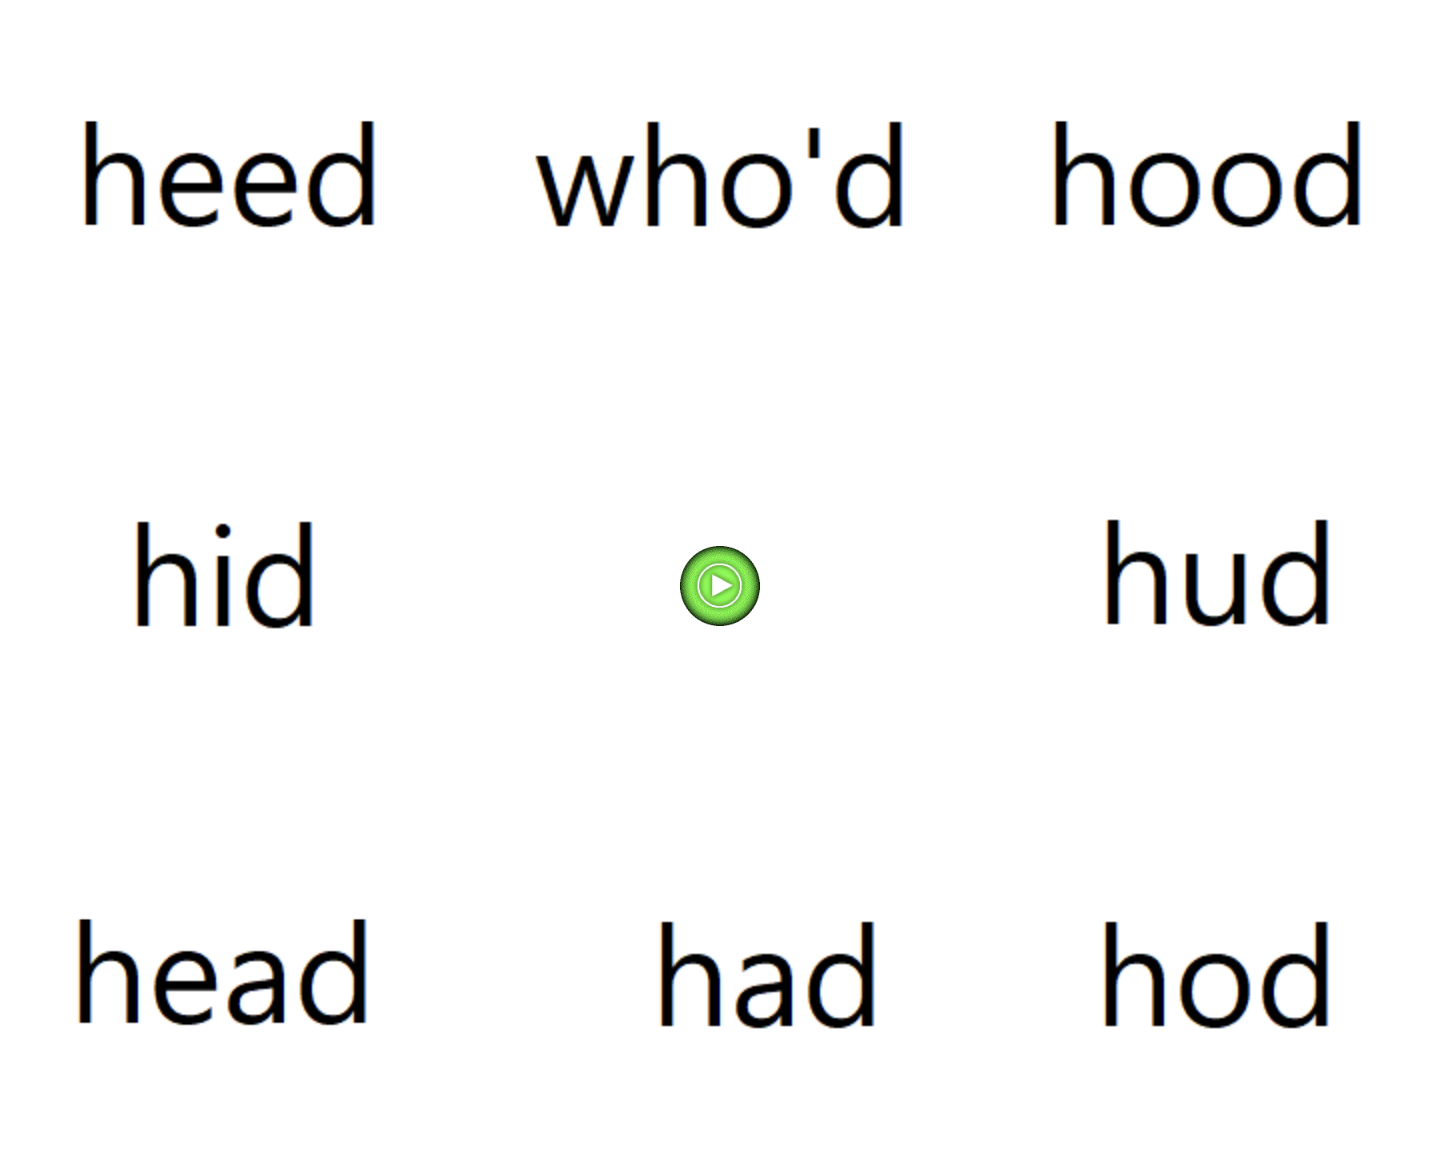
\includegraphics[width=0.4\linewidth]{figures/response-grid} 

}

\caption{Screen shot of the eight-alternative forced-choice (8-AFC) task used in both Experiment 1a and 1b.}\label{fig:exp-procedure}
\end{figure}

Experiment 1a employs recordings of \emph{hVd} word productions from a female talker of US English, these recordings are `natural' in the sense that they were not synthesized or otherwise phonetically manipulated. One consequence of this is that the formant values of these recordings are clustered around the \DIFaddbegin \DIFadd{talker's }\DIFaddend category means, and thus span only a comparatively small part of the phonetic space. This can limit the statistical power to distinguish between competing accounts. Natural recordings furthermore vary not only along the primary cues to vowel quality in US English (F1, F2) but also along \DIFdelbegin \DIFdel{potential }\DIFdelend secondary cues (e.g., F0, F3, \DIFdelbegin \DIFdel{and vowel duration}\DIFdelend \DIFaddbegin \DIFadd{vowel duration, and vowel inherent spectral change---VISC}\DIFaddend ) as well as other unknown properties, which can make it difficult to discern whether the performance of a normalization model is due to the normalization itself or other reasons, e.g., because a normalized cue happens to correlate with another cue that listeners are sensitive to but that is not included in the model.

Experiment 1b thus adopts an alternative approach and uses synthesized vowels. Unlike most previous work, which has used isolated vowels as stimuli \citep{barreda-nearey2012, barreda2021, nearey1989, richter2017}, Experiment 1b uses synthesized \emph{hVd} words to facilitate comparison to Experiment 1a. This allowed us to sample larger parts of the F1-F2 space, which has two advantages. First, it allowed us to collect responses over parts of the formant space for which we expect listeners to have more uncertainty, and thus exhibit more variable responses. This can increase the statistical power to distinguish between competing accounts. Second, differences in the predictions of competing normalization accounts will tend to become more pronounced with increasing distance from the category centers. By collecting responses at those locations, we can thus increase the contrast between competing accounts. \DIFaddbegin \DIFadd{Critically, an adequate model of formant normalization needs to capture human perception not only for prototypical vowel instances, but also instances of vowels that fall between category means.
}\DIFaddend 

The use of synthesized stimuli does, however, also come with potential disadvantages. Synthesized stimuli can suffer in ecological validity, lacking correlations between cues, and across the speech signal (e.g., due to co-articulation) that are characteristic of human speech. This raises questions about the extent to which processing of such stimuli engages the same mechanisms as everyday speech perception. Additionally, it is possible that the use of robotic sounding synthesized speech affects listener engagement. This can lead to an increased rate of attentional lapses, and thus a decrease in the proportion of trials on which listeners' responses are based on the acoustics of the speech stimulus rather than random guessing \citep[compare, e.g.,][]{kleinschmidt2020, tan-jaeger2024}. By comparing normalization accounts against both natural and synthesized stimuli, we investigate the extent to which the accounts that best describe human perception depend on the type of stimuli used in the experiment.

\subsection{Methods}\label{sec:methods}

\subsubsection{Participants}\label{sec:participants}

We recruited \DIFdelbegin \DIFdel{24 }\DIFdelend \DIFaddbegin \DIFadd{33 }\DIFaddend (Experiment 1a) and \DIFdelbegin \DIFdel{24 }\DIFdelend \DIFaddbegin \DIFadd{33 }\DIFaddend (Experiment 1b) participants\DIFaddbegin \DIFadd{. The majority of these (24 for each experiment) were recruited }\DIFaddend from Amazon's Mechanical Turk. \DIFaddbegin \DIFadd{However, after exclusions we were left with a relatively low number of participants (for Experiment 1a, 19, and for Experiment 1b, 22). We therefore decided to recruit an additional 18 participants from Prolific (9 for each experiment; October 2024). Exclusions described below left 28 and 31 participants for analysis in Experiments 1a and 1b, respectively. Results did not change after inclusion of the new participants from Prolific.
}

\DIFaddend Participants were paid \$6/hour \DIFaddbegin \DIFadd{(\$12/hour on Prolific) }\DIFaddend prorated by the duration of the experiments (15 minutes). Participants only saw the experiment advertised, and could only participate in it, if (i) they were located within the US, (ii) had an approval rating of 99\% or higher, (iii) met the software requirements (a recent version of the Chrome browser engine), and (iv) had not previously completed any other experiments on vowel perception in our lab. Before the experiment could be accepted, participants had to confirm that they were (i) native speakers of US English (defined as having spent their childhood until the age of 10 speaking English and living in the United States), (ii) in a quiet room without distractions, (\DIFdelbegin \DIFdel{ii}\DIFdelend \DIFaddbegin \DIFadd{iii}\DIFaddend ) wearing over-the-ear headphones. Participants' responses were collected via Javascript developed by the Human Language Processing Lab at the University of Rochester \citep{kleinschmidt2021}.

An optional post-experiment survey recorded participant demographics using NIH prescribed categories, including participant sex (Male: \DIFdelbegin \DIFdel{27}\DIFdelend \DIFaddbegin \DIFadd{36}\DIFaddend , Female: \DIFdelbegin \DIFdel{20}\DIFdelend \DIFaddbegin \DIFadd{29}\DIFaddend ), age (mean = \DIFdelbegin \DIFdel{35.5 }\DIFdelend \DIFaddbegin \DIFadd{36.9 }\DIFaddend years; SD = \DIFdelbegin \DIFdel{11.4}\DIFdelend \DIFaddbegin \DIFadd{12.2}\DIFaddend ; 95\% quantiles = \DIFdelbegin \DIFdel{24-63.25 }\DIFdelend \DIFaddbegin \DIFadd{22.6-66 }\DIFaddend years), race (White: \DIFdelbegin \DIFdel{36, Asian}\DIFdelend \DIFaddbegin \DIFadd{48, multiple}\DIFaddend : 3, Black: \DIFdelbegin \DIFdel{6, multiple: 1}\DIFdelend \DIFaddbegin \DIFadd{10, Asian: 3}\DIFaddend , declined to report: 1), and ethnicity (Non-Hispanic: \DIFdelbegin \DIFdel{42}\DIFdelend \DIFaddbegin \DIFadd{60}\DIFaddend , Hispanic: 4, declined to report: 1). \DIFaddbegin \DIFadd{All but 1 participant completed the survey.
}\DIFaddend 

\subsubsection{Materials}\label{sec:stimuli}

Experiment 1a employed \emph{hVd} word recordings by one adult female talker \DIFaddbegin \DIFadd{of a Northeastern dialect (spoken in central Connecticut) }\DIFaddend from a phonetically annotated database of L1-US English vowel productions \citep{xie-jaeger2020}. Specifically, we used all \DIFdelbegin \DIFdel{9 }\DIFdelend \DIFaddbegin \DIFadd{nine }\DIFaddend recordings of each of the eight \emph{hVd}-words---\emph{heed}, \emph{hid}, \emph{head}, \emph{had}, \emph{hut}, \emph{odd}, \DIFdelbegin \emph{\DIFdel{who'd}}%DIFAUXCMD
\DIFdel{, }\DIFdelend \emph{hood}\DIFaddbegin \DIFadd{, }\emph{\DIFadd{who'd}} \DIFaddend \citetext{\citealp[the use of ``hut'' and ``odd'' rather than ``hud'' and ``hod'' follows][]{assmann2008}; \citealp[but see][]{hillenbrand1995}}.

The stimuli for Experiment 1b were synthesized from a single \emph{had} recording used in Experiment 1a \DIFaddbegin \DIFadd{(see Figure \ref{fig:spectrograms} for example spectrograms)}\DIFaddend . Specifically, we used a script \citep[based on descriptions in][]{wade2007} in Praat \citep{boersma-weenink2022} to concatenate the original /h/ with a synthesized vowel and the original /d/ recording. Unlike in Experiment 1a, all eight words thus had an \emph{hVd} context (including ``hud'' and ``hod'', rather than ``hut'' and ``odd''). The Praat script first segmented the original \emph{had} token into \DIFaddbegin \DIFadd{the three segments }\DIFaddend /h/, /ae/ and /d/\DIFdelbegin \DIFdel{portions. It then filtered the }\DIFdelend \DIFaddbegin \DIFadd{, with the }\DIFaddend /\DIFaddbegin \DIFadd{d/ segment consisting of the voiced closure and burst. The script then estimated the spectral envelope of the /}\DIFaddend h/ sound \DIFdelbegin \DIFdel{inversely with its LPC}\DIFdelend \DIFaddbegin \DIFadd{by linear predictive coding (LPC; autocorrelation method), and used the resulting coefficients to inversely filter the /h/. This resulted in an /h/ sound with effects of vocal tract removed, leaving the source signal. Next, a glottal waveform was generated at each point in the pitch contour from the original /ae/ sound using the point process to phonation functionality in Praat. This waveform was multiplied with the intensity pattern from the same original /ae/ sound. The resulting sound was concatenated with the neutral fricative /h/ sound}\DIFaddend , \DIFdelbegin \DIFdel{and concatenated this neutral fricative sound with a complex waveform generated from the pitch and intensity patterns of the original vowel, }\DIFdelend to create a neutral hV-section that did not reflect any vocal tract resonances. The script then created a formant grid that filtered the hV-section to create the intended vowel, and finally concatenated this segment to the final /d/ to create an \emph{hVd} word. For each \emph{hVd} word, the formant grid was populated with the F1, F2 and F3 values that we handed to the script at five time-points transitioning from the /h/ to the \DIFaddbegin \DIFadd{steady-state }\DIFaddend vowel, to the \DIFaddbegin \DIFadd{first portion of the voiced closure of the }\DIFaddend final /d/ \DIFaddbegin \DIFadd{segment }\DIFaddend through linear interpolation\DIFaddbegin \DIFadd{, thus holding formants steady until transitioning into the final consonant}\DIFaddend . Formant bandwidths were 500 Hz at the initial two time-points (the /h/ and beginning of transition to vowel), and then decreased linearly during vowel onset and throughout the final three time-points to 50 Hz (F1), 100 Hz (F2), 200 Hz (F3), 300 Hz (F4), and 400 Hz \citep[F5-F8, following][]{wade2007}. The bandwidth manipulation implied that \DIFdelbegin \DIFdel{formants became stronger }\DIFdelend \DIFaddbegin \DIFadd{the spectral peaks of the formants became more defined and more separated }\DIFaddend as the vowel unfolded\DIFdelbegin \DIFdel{(see Figure \ref{fig:spectrograms})}\DIFdelend . We used this approach to create synthesized vowels for arbitrary F1-F2 combinations. F3 was set based on those F1-F2 values. Specifically, we ran a linear regression over the natural productions of the talker from Experiment 1a, predicting F3 from F1, F2 and their interaction. We then used that regression to predict F3 values for any F1-F2 combination in Experiment 1b. F4 to F8, as well as vowel duration, were held identical across all tokens \DIFdelbegin %DIFDELCMD < \citep[using the same values as][]{wade2007}%%%
\DIFdelend \DIFaddbegin \DIFadd{(using the automatically extracted vowel duration and mean formant values across the vowel segment from the }\emph{\DIFadd{had}} \DIFadd{token used for resynthesis)}\DIFaddend .



\begin{figure}

{\centering \subfloat[natural \emph{heed}\label{fig:spectrograms-1}]{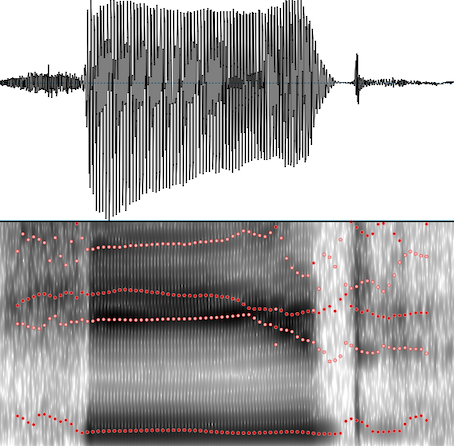
\includegraphics[width=0.2\linewidth]{figures/spectrogram_heed_1a} }\subfloat[natural \emph{hid}\label{fig:spectrograms-2}]{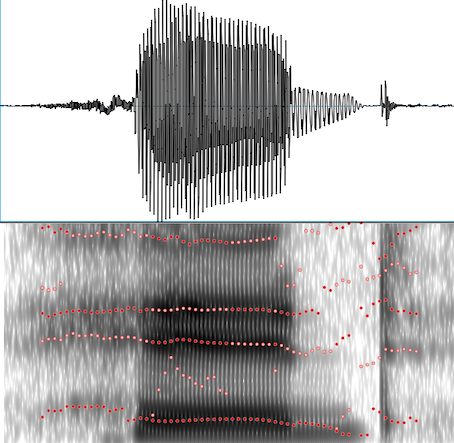
\includegraphics[width=0.2\linewidth]{figures/spectrogram_hid_1a} }\subfloat[natural \emph{odd}\label{fig:spectrograms-3}]{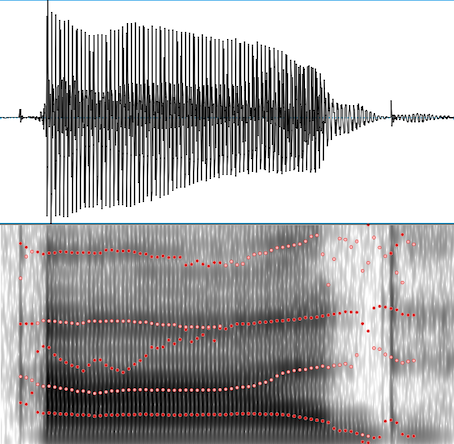
\includegraphics[width=0.2\linewidth]{figures/spectrogram_odd_1a} }\subfloat[natural \emph{hood}\label{fig:spectrograms-4}]{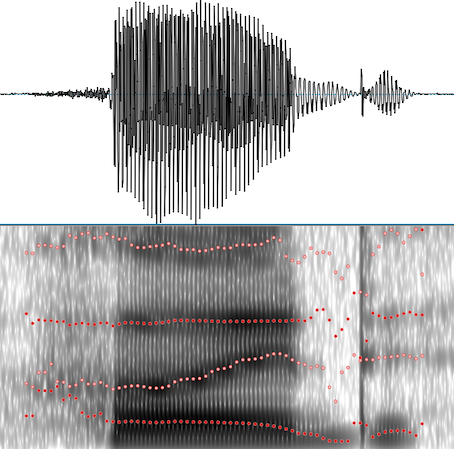
\includegraphics[width=0.2\linewidth]{figures/spectrogram_hood_1a} }\newline\subfloat[resynthesized \emph{heed}\label{fig:spectrograms-5}]{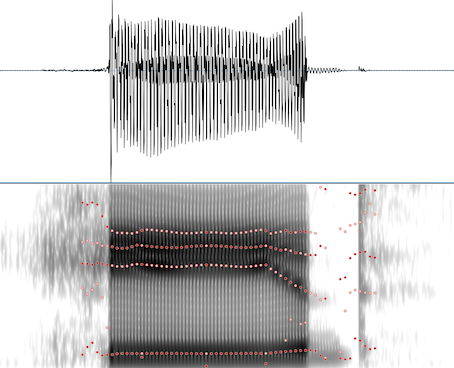
\includegraphics[width=0.2\linewidth]{figures/spectrogram_heed} }\subfloat[resynthesized \emph{hid}\label{fig:spectrograms-6}]{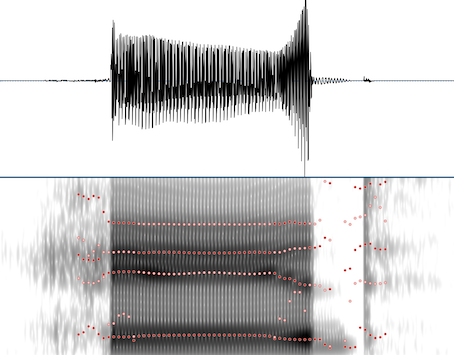
\includegraphics[width=0.2\linewidth]{figures/spectrogram_hid} }\subfloat[resynthesized \emph{hod}\label{fig:spectrograms-7}]{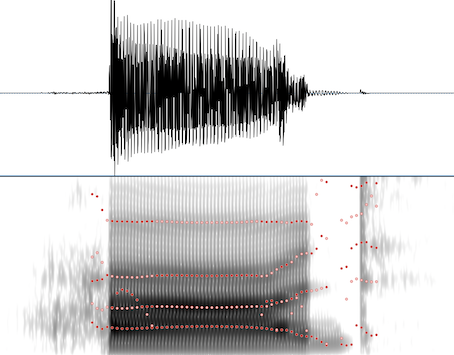
\includegraphics[width=0.2\linewidth]{figures/spectrogram_hod} }\subfloat[resynthesized \emph{hood}\label{fig:spectrograms-8}]{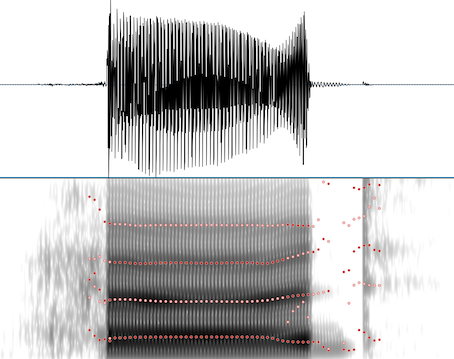
\includegraphics[width=0.2\linewidth]{figures/spectrogram_hood} }\newline

}

\caption{\textbf{Top:} Spectrograms of four natural recordings from Experiment 1a. \textbf{Bottom:} Same for four synthesized tokens with similar formant values from Experiment 1b. \DIFaddbeginFL \DIFaddFL{Additional spectrograms are provided in the SI \ref{sec:SI-spectrograms}.}\DIFaddendFL }\label{fig:spectrograms}
\end{figure}

We generated 146 synthesized \emph{hVd} recordings that spanned the F1 and F2 space. The specific F1-F2 locations chosen were determined by a mix of modeling (using ideal observers described in the next section to predict listeners' categorization responses) and intuition. Specifically, we selected 64 recordings that we expected to fall within the bivariate 95\% confidence intervals (CIs) of the eight US English monophthongs, and 82 recordings that we expected to fall between those CIs. Figure \ref{fig:human-performance} under \emph{Results} shows the distribution of stimuli for both experiments. Of note, our procedure also generated formant combinations that are physiologically unlikely to have all been produced by the same talker during `normal' vowel production \citep[also known as ``off-template'' instances,][]{nearey1978}.

\subsubsection{Procedure}\label{sec:procedure}

The procedure for both experiments was identical. Live instances of each experiment can be found at \url{https://www.hlp.rochester.edu/experiments/DLPL2S/experiment-A/experiments.html}. At the start of the experiment, participants acknowledged that they met all requirements and provided consent, as per the Research Subjects Review Board of the University of Rochester. Before starting the experiment, participants performed a sound check. Participants were then instructed to listen to a female talker saying words, and click on the word on screen to report what word they heard. On each trial, all eight \emph{hVd}-words were displayed on screen. Half of the participants in each experiment saw the response options organized as in Figure \ref{fig:exp-procedure} (resembling the IPA representation of a vowel space), half saw the response options in the opposite order (flipping top and bottom and left and right in Figure \ref{fig:exp-procedure}). Each trial started with the response grid on screen, together with a light green dot centered on screen. After 1000 ms, an \emph{hVd} recording played, and participants indicated their response by a mouse-click. After a 1000 ms intertrial interval, the screen reset, and the next trial started.

In both experiments, participants heard two blocks of the materials described in the previous sections, for a total of 144 trials in Experiment 1a and 292 trials in Experiment 1b. Presentation within each block was randomized for each participant \DIFaddbegin \DIFadd{in order to reduce confounds due to stimulus order }\citep[known to affect vowel perception,][ and references therein]{repp-crowder1990}\DIFaddend . Participants were not informed about the block structure of the experiment.

After completing the experiment, participants filled out a language background questionnaire and the optional demographic survey. On average, participants took \DIFdelbegin \DIFdel{10.3 }\DIFdelend \DIFaddbegin \DIFadd{9.3 }\DIFaddend minutes to complete Experiment 1a (SD = \DIFdelbegin \DIFdel{6.6) and 18.4 }\DIFdelend \DIFaddbegin \DIFadd{5.5) and 17.9 }\DIFaddend minutes for Experiment 1b (SD = \DIFdelbegin \DIFdel{7.3}\DIFdelend \DIFaddbegin \DIFadd{6.5}\DIFaddend ).

\subsubsection{Exclusions}\label{exclusions}

We excluded participants who failed to follow instructions and did not wear over-the-ear headphones (as indicated in the post-experiment survey). We also excluded participants with mean (log-transformed) reaction times that were unusually slow or fast (absolute z-score over by-participant means \textgreater{} 3), or if they clearly did not do the task (e.g., by answering randomly). This excluded \DIFdelbegin \DIFdel{6 }\DIFdelend \DIFaddbegin \DIFadd{5 }\DIFaddend participants from Experiment 1a and 2 from Experiment 1b (for details, see \DIFaddbegin \DIFadd{SI }\DIFaddend \ref{sec:SI-exclusions}).

We further excluded all trials that were unusually fast or slow. Specifically, we first z-scored the log-transformed response times \emph{within each participant} and then z-scored these z-scores \emph{within each trial} across participants. Trials with absolute z-scores \textgreater{} 3 were removed from analysis. This double-scaling approach was necessary as participants' response times decreased substantially over the first few trials and then continued to decrease less rapidly throughout the remainder of the experiment. The approach removes response times that are unusually fast or slow \emph{for that participant at that trial}, while avoiding specific assumptions about the shape of the speed up in response times across trials. This excluded \DIFdelbegin \DIFdel{1.2}\DIFdelend \DIFaddbegin \DIFadd{1.3}\DIFaddend \% of the trials in Experiment 1a and \DIFdelbegin \DIFdel{1.1}\DIFdelend \DIFaddbegin \DIFadd{0.9}\DIFaddend \% in Experiment 1b. This left for analysis \DIFdelbegin \DIFdel{2565 observations from 18 }\DIFdelend \DIFaddbegin \DIFadd{3983 observations from 28 }\DIFaddend participants in Experiment 1a, and \DIFdelbegin \DIFdel{6354 observations from 22 }\DIFdelend \DIFaddbegin \DIFadd{8970 observations from 31 }\DIFaddend participants in Experiment 1b.

\subsection{Results}\label{sec:experiment-results}

Participants' categorization responses in Experiments 1a and 1b are shown in Figure \ref{fig:human-performance}, with larger labels indicating recordings that participants agreed on more.\footnote{\citet{shannon1948} response entropy is defined as \(H(x) = -\sum_{i=1}^{n} P(x_{i}) \log P(x_{i})\). The maximum possible response entropy for an \DIFdelbegin \DIFdel{8-way }\DIFdelend \DIFaddbegin \DIFadd{eight-way }\DIFaddend response choice is 3 bits, which means that all eight vowels are responded equally often. The minimum response entropy = 0 bits, which means that the same vowel is responded all the time.} We make two observations. The first pertains to the degree of (dis)agreement between the two experiments. The second observation pertains to the degree of (dis)agreement across participants within each experiment.

\subsubsection{Similarities and differences between Experiments 1a and 1b}\label{similarities-and-differences-between-experiments-1a-and-1b}

\begin{figure}

{\centering \includegraphics[width=0.9\linewidth]{../../figures/knitted/human-performance} 

}

\caption{Summary of listeners' categorization responses in Experiments 1a and 1b in F1-F2 space. The vowel label indicates the most frequent response provided across participants on each test location. Size indicates how consistent responses were across participants, which larger symbols indicating more consistent responses (lower entropy). F1-F2 combinations below the gray dashed line are \DIFdelbeginFL \DIFdelFL{articulatory }\DIFdelendFL unlikely to \DIFdelbeginFL \DIFdelFL{come from }\DIFdelendFL \DIFaddbeginFL \DIFaddFL{be articulated by }\DIFaddendFL the same talker.}\label{fig:human-performance}
\end{figure}



Unsurprisingly, participants in both experiments divided the F1-F2 space into the eight vowel categories in ways that qualitatively resembled each other (after taking into account that Experiment 1b covers a larger range of F1-F2 values). Also unsurprisingly, there were some differences between participants' responses across the two experiments, at least when plotted in Hz. For example, {[}\ipatext{u}{]} rarely was the most frequent response in Experiment 1b, even for stimuli \DIFaddbegin \DIFadd{with similar F1-F2 values }\DIFaddend that were predominantly categorized as {[}\ipatext{u}{]} in Experiment 1a. There are at least two reasons to expect such differences. First, stimuli with similar F1-F2 values across the two experiments still differed in other acoustic properties (e.g.~vowel duration or F3). These acoustic differences might have affected participants' responses. Second, it is possible that \emph{formant normalization} affected participants' responses---i.e., the very mechanism we seek to investigate in the remainder of the paper. The two experiments differ in the means, variances, and other statistical properties that some normalization accounts predict to affect perception. As a consequence, Hz might not be the space in which we should expect identical responses across experiments.

Similarly, the two experiments differed in the extent to which participants agreed with each other. Participants in Experiment 1b exhibited overall less agreement in their responses (mean by-item response entropy = 0.45 bits, SE = 0.01) than participants in Experiment 1a (mean by-item response entropy = \DIFdelbegin \DIFdel{0.23 }\DIFdelend \DIFaddbegin \DIFadd{0.19 }\DIFaddend bits, SE = 0.02). This was \DIFdelbegin \DIFdel{expected given that }\DIFdelend \DIFaddbegin \DIFadd{also confirmed by participants' responses during the post-experiment survey. Compared to participants in Experiment 1a, participants in Experiment 1b reported increased uncertainty about their responses, and that the stimuli were less distinguishable and more robotic-sounding (see SI \ref{sec:SI-survey}).
}

\DIFadd{This increased uncertainty in }\DIFaddend Experiment 1b \DIFaddbegin \DIFadd{was expected---and, indeed, intended by the design: Experiment 1b }\DIFaddend explored the entire F1-F2 space, \DIFdelbegin \DIFdel{including---by design---formant }\DIFdelend \DIFaddbegin \DIFadd{including formant }\DIFaddend combinations located \emph{between} the centers of the natural vowel categories. Experiment 1b therefore achieved its goal of eliciting less categorical response distributions, which is expected to facilitate comparison of competing normalization accounts.\footnote{Note that participants in Experiment 1a exhibited high agreement on {[}\ipatext{ʌ}{]}, {[}\ipatext{æ}{]}, and {[}\ipatext{ɑ}{]}, despite the close proximity between, and partial overlap of, these vowels in F1-F2 space. To understand this pattern, it is important to keep in mind that the recordings for {[}\ipatext{ʌ}{]} and {[}\ipatext{ɑ}{]} differed from the recordings for other stimuli in their word onset (``odd'' for {[}\ipatext{ɑ}{]}) or offset (``hut'' for {[}\ipatext{ʌ}{]}).}

Auxiliary analyses presented in the SI (\ref{sec:SI-aux-entropy}) suggest that \emph{some but not all} of the differences in response entropy between the two experiments were caused by the placement of the stimuli in formant space: when comparing categorization responses for tokens from the two experiments with similar acoustic properties (differences of \(\le 30\) Hz along F1 and F2), response entropies still differed substantially (for N = 40 acoustically similar tokens, mean by-item response entropy for Experiment 1a = \DIFdelbegin \DIFdel{0.18 }\DIFdelend \DIFaddbegin \DIFadd{0.14 }\DIFaddend bits, SE = \DIFdelbegin \DIFdel{0.03}\DIFdelend \DIFaddbegin \DIFadd{0.02}\DIFaddend ; Experiment 1b = \DIFdelbegin \DIFdel{0.39 }\DIFdelend \DIFaddbegin \DIFadd{0.4 }\DIFaddend bits, SE = 0.03). \DIFaddbegin \DIFadd{The same section of the SI (\ref{sec:SI-aux-entropy}) presents additional analyses grouping acoustically similar tokens in the phonetic space defined by the normalization account we find to best fit listeners' responses. These analyses support the same conclusion.
}

\DIFaddend We see two mutually compatible explanations \DIFaddbegin \DIFadd{to this difference in listener agreement between experiments}\DIFaddend . First, similar to the differences between experiments in the dominant response pattern discussed above, differences in the degree of agreement between participants might originate in \emph{normalization}. Second, it is possible that the relation between formants in the synthesized stimuli or some other unknown acoustic-phonetic differences between the experiments explain the difference in response. For example, the absence of \DIFdelbegin \DIFdel{vowel inherent spectral change (VISC ) }\DIFdelend \DIFaddbegin \DIFadd{VISC }\DIFaddend or differences in \DIFaddbegin \DIFadd{spectral }\DIFaddend tilt in the synthesized stimuli might have deprived listeners of information that is actually crucial for establishing phonemic identity \citep{hillenbrand-nearey1999}. This would result in increased uncertainty on each trial, leading to increased entropy of listeners' responses. The computational study we present below shed some light on these two mutually compatible possibilities.

\subsubsection{Similarities and differences between participants}\label{similarities-and-differences-between-participants}

Since the intended category was known for Experiment 1a, it was possible to calculate participants' recognition accuracy. As also evident in the left panel of Figure \ref{fig:human-performance}, participants' most frequent response \emph{always} matched the intended vowel in Experiment 1a. Overall, participants' responses matched the intended vowel on \DIFdelbegin \DIFdel{81.2}\DIFdelend \DIFaddbegin \DIFadd{84.7}\DIFaddend \% (SE = \DIFdelbegin \DIFdel{4.8}\DIFdelend \DIFaddbegin \DIFadd{3.5}\DIFaddend \%) of all trials (Experiment 1b had no such ground truth). This is much higher than chance (12.5\%). It is, however, also quite a bit lower than 100\%. To better understand the reasons for this, Figure \ref{fig:human-confusion}A plots the confusion matrix. This suggests that participants' performance was largely affected by confusions between {[}\ipatext{ɪ}{]}-to-{[}\ipatext{ɛ}{]} (\emph{hid}-to-\emph{head}), {[}\ipatext{ɛ}{]}-to-{[}\ipatext{æ}{]} (\emph{head}-to-\emph{had}), and {[}\ipatext{u}{]}-to-{[}\ipatext{ʊ}{]} (\emph{who'd}-to-\emph{hood}).



\begin{figure}[!ht]

{\centering \includegraphics[width=0.9\linewidth]{../../figures/knitted/human-confusion} 

}

\caption{Category confusability in Experiments 1a and 1b. \textbf{Panel A} summarizes the category confusability. Since correct responses were not defined for Experiment 1b, we grouped items along the x-axis based on most frequent response that listeners provided (for Experiment 1a, this was always identical to the intended response). Response percentages sum to 100 in each column, showing the response distribution depending on the most frequent response. \textbf{Panel B} summarizes individual differences across listeners, in terms of the listener-specific confusability of {[}\ipatext{ɪ}{]} with {[}\ipatext{ɛ}{]} (x-axis), {[}\ipatext{ɛ}{]} with {[}\ipatext{æ}{]} (y-axis), and {[}\ipatext{u}{]} with {[}\ipatext{ʊ}{]} (color fill).}\label{fig:human-confusion}
\end{figure}

One plausible explanation for this pattern of vowel confusions lies in the substantial variation that exists across US English dialects \citep{atlasnae}. Differences in the realization of vowel categories, and associated representations, across dialects will directly affect the expected classification for any given token. In addition, listeners might differ in terms of experience with different dialects, or in the dialect they attribute to the talker who produced the stimuli. To test this hypothesis, we calculated the {[}\ipatext{ɪ}{]}-to-{[}\ipatext{ɛ}{]}, {[}\ipatext{ɛ}{]}-to-{[}\ipatext{æ}{]}, and {[}\ipatext{u}{]}-to-{[}\ipatext{ʊ}{]} confusion rates for each participant in Experiment 1a. These data are summarized in the left panel of Figure \ref{fig:human-confusion}B. The data in the left panel suggest that most participants in Experiment 1a either heard {[}\ipatext{ɪ}{]} tokens consistently as the intended {[}\ipatext{ɪ}{]} (clustering on the left side of the panel) or as {[}\ipatext{ɛ}{]} (clustering on the right side of the panel). Only a few participants exhibited mixed responses for items intended to be {[}\ipatext{ɪ}{]}. Tellingly, many of the participants who exhibited increased {[}\ipatext{ɪ}{]}-to-{[}\ipatext{ɛ}{]} confusion \emph{also} exhibited increased {[}\ipatext{ɛ}{]}-to-{[}\ipatext{æ}{]} confusion. This is precisely what would be expected by listeners who assume a dialect in which these vowels are articulated lower (with higher F1) than in the dialect of the talker in Experiment 1a. A similar, but less pronounced, pattern was also found with regard to {[}\ipatext{u}{]}-to-{[}\ipatext{ʊ}{]} confusions.\footnote{{[}\ipatext{u}{]} has been undergoing changes in many varieties of US English. Whereas the talker in Experiment 1a produces {[}\ipatext{u}{]} with low F1 and F2 (high and back), other L1 talkers of US English produce this vowel considerably more forward (higher F2).} Finally, a qualitatively similar relation between {[}\ipatext{ɪ}{]}-to-{[}\ipatext{ɛ}{]}, {[}\ipatext{ɛ}{]}-to-{[}\ipatext{æ}{]}, and {[}\ipatext{u}{]}-to-{[}\ipatext{ʊ}{]} confusions was also observed in Experiment 1b (right panel of Figure \ref{fig:human-confusion}B), though the pattern was unsurprisingly less pronounced given that the stimuli in Experiment 1b by design often fell into the ambiguous region \emph{between} vowels. Taken together, \DIFaddbegin \DIFadd{vowel-to-vowel confusion rates in }\DIFaddend Experiments 1a and 1b \DIFdelbegin \DIFdel{thus }\DIFdelend suggest that systematic dialectal differences \DIFdelbegin \DIFdel{between participants may be a substantial contributor of }\DIFdelend \DIFaddbegin \DIFadd{contributed to }\DIFaddend the relatively low \DIFdelbegin \DIFdel{correct classification rate observed for Experiment 1a}\DIFdelend \DIFaddbegin \DIFadd{categorization accuracy}\DIFaddend .

This highlights two important points. First, the data from Experiment 1a demonstrate the perceptual challenges associated with an unfamiliar talker: in the absence of lexical or other context to distinguish between the eight available response options, listeners can only rely on the acoustic information in the input. In such a scenario, even listeners who are in principle familiar with the dialect spoken by the talker have comparatively little information to determine the talker's dialect, making apparent what \DIFdelbegin \DIFdel{Matt }\DIFdelend \citet{winn2018} aptly summarizes as ``speech {[}perception{]} is not as acoustic as {[}we{]} think''. Second, when dialect variability is taken into account, listeners' recognition accuracy improved substantially. After removing \DIFdelbegin \DIFdel{7 }\DIFdelend \DIFaddbegin \DIFadd{8 }\DIFaddend listeners who heard more than 50\% of the {[}\ipatext{ɪ}{]} items as {[}\ipatext{ɛ}{]}, \emph{all} vowels were correctly recognized at least \DIFdelbegin \DIFdel{88.3}\DIFdelend \DIFaddbegin \DIFadd{87.1}\DIFaddend \% of the time (overall accuracy = \DIFdelbegin \DIFdel{95.9}\DIFdelend \DIFaddbegin \DIFadd{94.8}\DIFaddend \%). This suggests that dialect differences affected the recognition of all vowels. This aspect of our results serves as an important reminder that formant normalization is only expected to erase inter-talker variability associated with \emph{physiological} differences: variation in dialect, sociolect, or other non-physiologically-conditioned variation pose separate challenges to human perception, and require additional mechanisms \citep[see discussion in][]{barreda2021, weatherholtz-jaeger2016}. This introduces noise---variability in listeners' responses that cannot be accounted for by normalization---to any comparison of normalization accounts, potentially reducing the power to detect differences between accounts.

\section{Comparison of normalization accounts}\label{comparison-of-normalization-accounts}

In order to evaluate normalization accounts against speech perception, it is necessary to map the phonetic properties of stimuli---under different hypotheses about normalization---onto listeners' responses in Experiments 1a and 1b. Previous work has done so by directly predicting listeners' responses from the raw or normalized phonetic properties of stimuli \citep{apfelbaum-mcmurray2015, barreda2021, crinnion2020, mcmurray-jongman2011, nearey1989}. For example, McMurray and Jongman used multinomial logistic regression to predict \DIFdelbegin \DIFdel{8-way }\DIFdelend \DIFaddbegin \DIFadd{eight-way }\DIFaddend fricative categorization responses in US English \citep[see also][]{barreda2021}.

Here we pursued an alternative approach by committing to a core assumption common to contemporary theories of speech perception: that listeners acquire implicit knowledge about the probabilistic mapping from acoustic inputs to linguistic categories, and draw on this knowledge during speech recognition \citetext{\citealp[e.g., TRACE,][]{mcclelland-elman1986}; \citealp[exemplar theory,][]{johnson1997}; \citealp[Bayesian accounts,][]{luce-pisoni1998}; \citealp{nearey1990}; \citealp{norris-mcqueen2008}; \citealp[ASR-inspired models like DIANA or EARSHOT,][]{bosch2015}; \citealp{magnuson2020}}. Using a general computational framework for adaptive speech perception \citep[ASP,][]{xie2023} we trained Bayesian ideal observers to capture the expectations that a `typical' L1 adult listener might have about the formant-to-vowel mappings of US English. We approximated these expectations using a database of L1-US English vowel productions \citep{xie-jaeger2020}---transformed to reflect the different normalization accounts. We then ask which of the different ideal observer models---corresponding to different hypotheses about formant normalization---best predicts listeners' responses in Experiments 1a and 1b.

\DIFdelbegin \DIFdel{A welcome side effect of this is that far fewer }\DIFdelend \DIFaddbegin \DIFadd{Training ideal observers on a database of vowel productions has the advantage that it reduces the }\DIFaddend degrees of freedom (DFs) \DIFdelbegin \DIFdel{are required }\DIFdelend \DIFaddbegin \DIFadd{used }\DIFaddend to predict listeners' responses. For example, using ordinary multinomial logistic regression trained on our perceptual data to predict \DIFdelbegin \DIFdel{8-way }\DIFdelend \DIFaddbegin \DIFadd{eight-way }\DIFaddend vowel categorization as a function of F1, F2 and their interaction would require up to 28 DFs. This problem increases with the number of cues considered. \DIFdelbegin \DIFdel{Because the model is trained on data that is independent of our perceptual data}\DIFdelend \DIFaddbegin \DIFadd{By instead training ideal observers on phonetic data that are independent of listeners' responses}\DIFaddend , the ASP-based approach we employ \DIFdelbegin \DIFdel{instead uses only 2 DFs (i.e., parameters estimated based on our perceptual data) }\DIFdelend \DIFaddbegin \DIFadd{uses only two DFs }\DIFaddend to mediate the mapping from stimuli properties to listeners' responses, regardless of the number of cues considered. Over the next few sections, we describe how this parsimony is made possible through a commitment to strong linking hypotheses motivated by theories of speech perception.

\subsection{Methods}\label{methods}

\subsubsection{\texorpdfstring{A general-purpose categorization model for \(J\)-AFC categorization tasks}{A general-purpose categorization model for J-AFC categorization tasks}}\label{sec:predict-perception}

\begin{figure}[!ht]
\begin{center}
   \DIFdelbeginFL %DIFDELCMD < \tikz{ %
%DIFDELCMD <     \node[obs] (r) {$r$} ; %
%DIFDELCMD <     \node[const, right=of r, xshift=-.009cm] (r_description) {{\em categorization response}} ; %
%DIFDELCMD <     \node[det, below=of r] (decision) {} ; %
%DIFDELCMD < % decisions
%DIFDELCMD <     \node[const, right=of decision, xshift=-.009cm] (decision_rule) {{\em decision rule} (Luce choice rule)} ; %
%DIFDELCMD <     \factor[below=of decision, xshift=-.009cm, yshift=-.5cm] {response-dist} {left: $\mathcal{M}$} {} {}; %
%DIFDELCMD <     \factor[right=of response-dist, xshift=.8cm, yshift=-1cm] {prior-dist} {left: Multi} {} {}; %
%DIFDELCMD <     \factor[below=of response-dist, xshift=-.009cm, yshift=-1cm] {multi} {left: Multi} {} {}; %
%DIFDELCMD <     \node[latent, right=of response-dist, xshift=1.5cm] (l) {$\lambda$} ; %
%DIFDELCMD <     \node[const, right=of l, xshift=-.009cm] (lapse) {{\em lapse rate} ($1$ DF)} ; %
%DIFDELCMD <     \node[latent, right=of prior-dist, xshift=.2cm, yshift=-.009cm] (pi_n) {$\pi_{c}$} ; %
%DIFDELCMD <     \node[right=of pi_n] (beta_description) {{\em response biases}} ;
%DIFDELCMD < % edges
%DIFDELCMD <     \edge {decision} {r} ;
%DIFDELCMD <     \edge {response-dist} {decision} ; %
%DIFDELCMD <     \edge {multi} {response-dist} ; %
%DIFDELCMD <     \edge {prior-dist} {response-dist} ; %
%DIFDELCMD <     \edge {prior-dist} {multi} ; %
%DIFDELCMD <     \edge {l} {response-dist} ; %
%DIFDELCMD <     \edge {pi_n} {prior-dist} ;
%DIFDELCMD < % representations
%DIFDELCMD <     \factor[below=of multi,  yshift=-1cm] {x_prime} {left:$\mathcal{N}$} {} {}; %
%DIFDELCMD <      %\node[above=of x_prime] (dots) {$\vdots$} ; %
%DIFDELCMD <     \node[obs, right=of x_prime, yshift=.5cm, xshift=.3cm] (mu_n) {$\mu_{c}$} ; %
%DIFDELCMD <     \node[obs, right=of x_prime, yshift=-.5cm, xshift=.3cm] (sigma_n) {$\Sigma_{c}$} ; %
%DIFDELCMD <     \node[right=of mu_n] (mu_n_description) {{\em category means} (estimated from phonetic database)} ;
%DIFDELCMD <     \node[right=of sigma_n] (sigma_n_description) {{\em category covariance} (estimated from phonetic database)} ;
%DIFDELCMD < 

%DIFDELCMD < % edges
%DIFDELCMD <     \edge {x_prime} {multi} ; %
%DIFDELCMD <     \edge {mu_n} {x_prime} ; %
%DIFDELCMD <     \edge {sigma_n} {x_prime} ; %
%DIFDELCMD < % noise
%DIFDELCMD <     \node[det, below=of x_prime, yshift=-1cm] (x_prime2) {} ; %
%DIFDELCMD <       %\node[above=of x_prime2] (dots) {$\vdots$} ; %
%DIFDELCMD <     \node[latent, right=of x_prime2] (sigma_noise) {$\Sigma_{noise}$} ; %
%DIFDELCMD <     \node[right=of sigma_noise, xshift=-.3cm] (sigma_noise_description) {{\em internal \& external noise} (1 DF)} ;
%DIFDELCMD < %edges
%DIFDELCMD <     \edge {x_prime2} {x_prime} ; %
%DIFDELCMD <     \edge {sigma_noise} {x_prime2} ; %
%DIFDELCMD < % normalization
%DIFDELCMD <     \node[det, below=of x_prime2, yshift=-.4cm] (x_prime3) {} ; %
%DIFDELCMD <     \node[obs, right=of x_prime3] (theta) {$\theta$} ; %
%DIFDELCMD <     \node[right=of theta] (theta_description) {{\em normalization parameters} (estimated from phonetic database \& stimuli)} ; %
%DIFDELCMD <     \node[obs, below=of x_prime3] (x) {x} ; %
%DIFDELCMD <     \node[const, right=of x, xshift=-.009cm] (x_description) {{\em phonetic properties of stimulus} (formants)} ;
%DIFDELCMD < %edges
%DIFDELCMD <     \edge {x_prime3} {x_prime2} ; %
%DIFDELCMD <     \edge {theta} {x_prime3} ; %
%DIFDELCMD <     \edge {x} {x_prime3} ; %
%DIFDELCMD < }
%DIFDELCMD < %%%
\DIFdelendFL \DIFaddbeginFL \tikz{ %
    \node[obs] (r) {$r$} ; %
    \node[const, right=of r, xshift=-.009cm] (r_description) {{\em categorization response}} ; %
    \node[det, below=of r] (decision) {} ; %
% decisions
    \node[const, right=of decision, xshift=-.009cm] (decision_rule) {{\em decision rule} (Luce choice rule)} ; %
    \factor[below=of decision, xshift=-.009cm, yshift=-.5cm] {response-dist} {left: $\mathcal{M}$} {} {}; %
    \factor[right=of response-dist, xshift=.8cm, yshift=-1cm] {prior-dist} {left: Multi} {} {}; %
    \factor[below=of response-dist, xshift=-.009cm, yshift=-1cm] {multi} {left: Multi} {} {}; %
    \node[latent, right=of response-dist, xshift=1.5cm] (l) {$\lambda$} ; %
    \node[const, right=of l, xshift=-.009cm] (lapse) {{\em lapse rate} ($1$ DF)} ; %
    \node[latent, right=of prior-dist, xshift=.2cm, yshift=-.009cm] (pi_n) {$\pi_{c}$} ; %
    \node[right=of pi_n] (beta_description) {{\em response biases}} ;
% edges
    \edge {decision} {r} ;
    \edge {response-dist} {decision} ; %
    \edge {multi} {response-dist} ; %
    \edge {prior-dist} {response-dist} ; %
    \edge {prior-dist} {multi} ; %
    \edge {l} {response-dist} ; %
    \edge {pi_n} {prior-dist} ;
% representations
    \factor[below=of multi,  yshift=-1cm] {x_prime} {left:$\mathcal{N}$} {} {}; %
     %\node[above=of x_prime] (dots) {$\vdots$} ; %
    \node[obs, right=of x_prime, yshift=.5cm, xshift=.3cm] (mu_n) {$\mu_{c}$} ; %
    \node[obs, right=of x_prime, yshift=-.5cm, xshift=.3cm] (sigma_n) {$\Sigma_{c}$} ; %
    \node[right=of mu_n] (mu_n_description) {{\em category means} (estimated from phonetic database)} ;
    \node[right=of sigma_n] (sigma_n_description) {{\em category covariance} (estimated from phonetic database)} ;

% edges
    \edge {x_prime} {multi} ; %
    \edge {mu_n} {x_prime} ; %
    \edge {sigma_n} {x_prime} ; %
% noise
    \node[det, below=of x_prime, yshift=-1cm] (x_prime2) {} ; %
      %\node[above=of x_prime2] (dots) {$\vdots$} ; %
    \node[latent, right=of x_prime2] (sigma_noise) {$\Sigma_{noise}$} ; %
    \node[right=of sigma_noise, xshift=-.3cm] (sigma_noise_description) {{\em internal \& external noise} (1 DF)} ;
%edges
    \edge {x_prime2} {x_prime} ; %
    \edge {sigma_noise} {x_prime2} ; %
% normalization
    \node[det, below=of x_prime2, yshift=-.4cm] (x_prime3) {} ; %
    \node[obs, right=of x_prime3] (theta) {$\theta$} ; %
    \node[right=of theta] (theta_description) {{\em normalization parameters} (estimated from phonetic database \& stimuli)} ; %
    \node[obs, below=of x_prime3] (x) {x} ; %
    \node[const, right=of x, xshift=-.009cm] (x_description) {{\em acoustic properties of stimulus} (formants)} ;
%edges
    \edge {x_prime3} {x_prime2} ; %
    \edge {theta} {x_prime3} ; %
    \edge {x} {x_prime3} ; %
}
\DIFaddendFL 

\caption{Graphical model of ASP's general categorization framework (adapted for the current purpose from Xie et al., 2023, Figure 4). Here $J=8$ (the eight vowel response options in Experiments 1a and 1b). We use this framework to compare normalization accounts against listeners' categorization responses from Experiments 1a and 1b. Filled gray circles represent variables that are known to the researcher. Empty circles represent latent variables that are not observable. Diamonds represent variable-free processes, annotated with the distributions resulting at that level of the model: $\mathcal{N}$(ormal), Multi(nomial), and $\mathcal{M}$(ixture) distributions.} \label{fig:model-perceptual-decision-making}
\end{center}
\end{figure}

Figure \ref{fig:model-perceptual-decision-making} summarises ASP's categorization model for a \(J\)-alternative forced-choice task \citep[for an in-depth description, we refer to][]{xie2023}. The model combines Bayesian ideal observers \citetext{\citealp[as used in e.g.,][]{clayards2008}; \citealp{feldman2009}; \citealp{norris-mcqueen2008}; \citealp{xie2021}; \citealp[for a closely related approach, see also][]{nearey-hogan1986}} with psychometric lapsing models \citep{wichmann-hill2001}. To reduce researchers' degrees of freedom, we adopt all assumptions made in \citet{xie2023}, and do not introduce additional assumptions.

Starting at the bottom of the figure, the \DIFdelbegin \DIFdel{phonetic }\DIFdelend \DIFaddbegin \DIFadd{acoustic }\DIFaddend input \(x\) is normalized. Here, \DIFaddbegin \DIFadd{we follow most previous evaluations of normalization accounts, and focus on the point estimates of formants at the center of the vowel as the inputs to normalization. This leaves open the question of how considerations of additional cues to vowel identity (e.g., VISC) or formant dynamics might affect the findings we report below (a point to which we return in the general discussion). Specifically, the main analysis we present here focus on }\DIFaddend \(x\) = \DIFdelbegin \DIFdel{the }\DIFdelend F1 and F2\DIFdelbegin \DIFdel{of our stimuli (the }\DIFdelend \DIFaddbegin \DIFadd{. As one anonymous reviewer pointed out, this focus on F1-F2 might underestimate the potential of }\emph{\DIFadd{intrinsic}} \DIFadd{normalization accounts, which might perform better when more acoustic-phonetic features are considered. The }\DIFaddend SI, \ref{sec:SI-F1F3}\DIFaddbegin \DIFadd{, thus }\DIFaddend reports additional analyses that instead employ F1-F3\DIFdelbegin \DIFdel{; these analyses support the same conclusion presented here, and we mention them below where relevant).
}\DIFdelend \DIFaddbegin \DIFadd{. These analyses indeed find that the fit of intrinsic normalization accounts improves more than that of extrinsic accounts when F3 is included in the analysis. However, the best-fitting accounts were still the same extrinsic accounts we find to best fit listeners' responses when only F1 and F2 is considered.
}

\DIFaddend The specific computations applied to the input \(x\) depend on the normalization accounts (see Table \ref{tab:norm-accounts}). We use \(\theta\) to refer to the parameters required by the normalization account. For example, for \DIFdelbegin \DIFdel{the }\DIFdelend \DIFaddbegin \DIFadd{Nearey's }\DIFaddend uniform scaling account \citep{nearey1978}, \(\theta\) is the overall mean of all log-transformed formants. For Lobanov normalization \citep{lobanov1971}, \(\theta\) is a vector of means and standard deviations for each formant (in Hz). \DIFdelbegin %DIFDELCMD < 

%DIFDELCMD < %%%
\DIFdelend The normalized input is then perturbed by perceptual and environmental noise. Following \citet{feldman2009}, this noise is assumed to be Gaussian distributed centered around the transformed stimulus with noise variances that are independent and identical for all formants (i.e., \(\Sigma_{noise}\) is a diagonal matrix, and all diagonal entries have the same value).
\DIFaddbegin 

\DIFaddend Next, the likelihood of the normalized percept under each of the eight vowel categories is calculated, \(p(F1, F2 | vowel)\). This requires specifying listeners' expectations about the cue-to-category mapping (listeners' likelihood function). We followed \citet{xie2023} and previous work and assume that each vowel maps onto a multivariate Gaussian distribution over the phonetic cues, here bivariate Gaussians over F1 and F2 \citep[cf.][]{clayards2008, feldman2009, kleinschmidt-jaeger2015, norris-mcqueen2008, xie2021}. \DIFdelbegin \DIFdel{The }\DIFdelend \DIFaddbegin \DIFadd{We also followed previous models in assuming a single dialect template---i.e., a single set of bivariate Gaussian vowel categories }\citep{nearey-assmann2007}\DIFadd{. The analyses of participants' responses we provided above in the description of Experiments 1a and 1b suggest that this assumption is wrong. However, more appropriate alternatives---such as hierarchical or mixture models with multiple dialect templates---will require substantial additional research as well as larger databases of vowel recordings that have high resolution both within and across dialects. We return to this issue in the general discussion.
}

\DIFadd{Once the likelihood function for each vowel is specified, the }\DIFaddend posterior probability of each vowel is obtained by combining its likelihood with its prior probability or response bias \(\pi_c\), according to Bayes theorem:\footnote{For Gaussian noise and Gaussian category likelihoods, the resulting noise-convolved likelihood is a Gaussian with variance equal to the sum of the noise and category variances \citep{kronrod2016}.}

\begin{equation}
 p(vowel = c |F1, F2) = \frac{\mathcal{N}(F1, F2| \mu_c, \Sigma_c + \Sigma_{noise}) \times \pi_c}{\sum_{c_i} \mathcal{N}(F1, F2|\mu_{c_i}, \Sigma_{c_i} + \Sigma_{noise}) \times \pi_{c_i}} \label{eq:Bayes-rule-normal}
\end{equation}

Up to this point, the model is identical to a standard Bayesian ideal observer over noisy input \citep{feldman2009, kronrod2016} for which the input has been transformed based on the normalization account. ASP's categorization model adds to this the potential that participants experience attentional lapses---or for other reasons do not respond based on the input---on some proportion of all trials \citep[\(\lambda\), as in standard psychometric lapsing models,][]{wichmann-hill2001}. On those trials, the posterior probability of a category is determined solely by participants' response bias, which we assume to be identical to the response bias on non-lapsing trials \citep[following][]{xie2023}. This results in a posterior that is described by weighted mixture of two components, describing participants' posterior on non-lapsing and lapsing trials, respectively:

\begin{equation}
 p(vowel = v|F1, F2) = (1-\lambda) \frac{\mathcal{N}(F1, F2| \mu_c, \Sigma_c + \Sigma_{noise}) \times \pi_c}{\sum_{c_i} \mathcal{N}(F1, F2|\mu_{c_i}, \Sigma_{c_i} + \Sigma_{noise}) \times \pi_{c_i}} + \lambda \frac{\pi_c}{\pi_{c_i}} \label{eq:Bayes-rule-ASP}
\end{equation}

Finally, a decision rule is applied to the posterior to determine the response of the model, conditional on the input (one of the eight vowels in Experiments 1a and 1b). We followed the gross of research on speech perception and assume Luce's choice rule \citetext{\citealp{luce1959}; \citealp[for discussion, see][]{massaro-friedman1990}}. Under this choice rule, the model can be seen as sampling from the posterior, responding with each category proportional to that category's posterior probability.

Next, we describe how we estimated the \(\theta\)s, \(\mu_c\)s and \(\Sigma_c\)s for each normalization account from a phonetic database. We use this database as a---very coarse-grained---approximation of a the speech input a `typical' listener might have experienced previously. By fixing \(\theta\), \(\mu_c\) and \(\Sigma_c\) based on the distribution of phonetic cues in the database, we substantially reduce the DFs that are allowed to mediate the mapping from stimulus properties to listeners' responses \citep[following][]{xie2023}. In addition, this approach naturally penalizes overly complex models by validating these against out-of-sample data. Finally, we describe how we fit the remaining parameters as DFs to participants' responses from Experiments 1a and 1b.

\subsubsection{\texorpdfstring{Modeling listeners' prior experience (and guarding against overfitting): \(\theta\), \(\mu_c\), and \(\Sigma_c\)}{Modeling listeners' prior experience (and guarding against overfitting): \textbackslash theta, \textbackslash mu\_c, and \textbackslash Sigma\_c}}\label{modeling-listeners-prior-experience-and-guarding-against-overfitting-theta-mu_c-and-sigma_c}

By fixing \(\theta\), \(\mu_c\), and \(\Sigma_c\) based on a database of vowel \emph{productions}, we impose strong constraints on the functional flexibility of the model in predicting listeners' responses. This benefit is made possible by committing to a strong linking hypothesis---that listeners' categories are learned from, and reflect, the distributional mapping from formants to vowels in previously experienced speech input \citep[e.g.,][]{abramson-lisker1973, massaro-friedman1990, nearey-hogan1986}. The database we use to approximate listeners' prior experience was originally developed to compare the production of L1 and L2 speakers \citep{xie-jaeger2020}. It contains 9-10 recordings of the \DIFdelbegin \DIFdel{8 }\DIFdelend \DIFaddbegin \DIFadd{eight }\DIFaddend \emph{hVd} words from each of 17 (\DIFdelbegin \DIFdel{5 }\DIFdelend \DIFaddbegin \DIFadd{five }\DIFaddend female) L1 talkers of a Northeastern dialect of US English (ages 18 to 35 years old). Since Experiments 1a and 1b used recordings of one of these talkers, we excluded that talker prior to fitting training ideal observers on the data. In total, this yields 5842 recordings that are annotated for F0, F1-F3, and vowel duration. The SI (\ref{sec:SI-xie-jaeger}) summarizes the distribution of these cues, and how the different normalization accounts affect those distributions.

To avoid over-fitting the ASP model to the database, we used 5-fold cross-validation: we randomly split the \citet{xie-jaeger2020} database into five approximately evenly-sized folds \citep[following][]{persson-jaeger2023}. This split was performed within each vowel to guarantee that all five folds had the same relative amount of data for each vowel category. These splits were combined into five training sets, each containing one of the folds (20\% of the data). This way, each training set was different from the others, increasing the variability between sets.\footnote{We intentionally did \emph{not} split the data within talkers since normalization accounts are meant to make speech perception robust to cross-talker variability. Further, splitting the data by speaker rather than by vowel category avoids the potential for biases in the normalization parameter estimates for different speakers in the case of missing or unbalanced tokens across vowel categories, see \citep{barreda-nearey2018}. Additional analyses not reported here confirmed that the same results are obtained when splits are performed within talkers and within vowels (except that this lead to smaller CIs, and thus \emph{more} significant differences, in Figure \ref{fig:plot-io-optimal}). These analyses can be replicated by downloading the R markdown document this article is based on from our OSF (see comments in our code).}

For each training set and for each normalization account, we then estimated the required normalization parameters \(\theta\) for all talkers, and normalized all formants based on those talker-specific parameters. This yielded 5 (training sets) * 20 (accounts) = 100 normalized training sets. For each of these normalized training sets, we fit the category means, \(\mu_c\), and covariance matrices, \(\Sigma_c\), of all eight vowels, using the \texttt{R} package \texttt{MVBeliefUpdatr} \citep{R-MVBeliefUpdatr}.\footnote{Alternatively, it would be possible to treat these parameters as DFs in the link to listeners' responses, and infer them from the responses in Experiments 1a and 1b \citep[cf.,][]{kleinschmidt-jaeger2016}. This approach would afford the model with a high degree of functional flexibility, regardless of which normalization approach is applied (similar to previous approaches that have employed, e.g., multinomial logistic regression).}

This yielded 100 ideal observer models, \DIFdelbegin \DIFdel{5 }\DIFdelend \DIFaddbegin \DIFadd{five }\DIFaddend for each of the 20 normalization accounts in Table \ref{tab:norm-accounts}. Of note, the 20 ideal observers fit on each fold differ \emph{only} in the assumptions they make about the normalization that is applied to cues before they are mapped onto the eight vowel categories. Figure \ref{fig:io-plot-categories} visualizes the resulting bivariate Gaussian categories for four of the 20 normalization accounts. This illustrates one advantage of the cross-validation approach: it takes a modest step towards simulating differences across listeners' prior experience (represented by the five different folds).



\begin{figure}[!ht]

{\centering \includegraphics[width=0.95\linewidth]{../../figures/knitted/io-plot-categories} 

}

\caption{Visualizing the bivariate Gaussian categories (prior to adding \(\Sigma_{noise}\)) of four example normalization accounts in F1-F2 space. Separate ellipses are shown for each of the five training sets (each set corresponds to one set of eight ellipses). The relative stability of the category ellipses across training sets indicates that the database is sufficiently large for the present purpose.}\label{fig:io-plot-categories}
\end{figure}

\subsubsection{Transforming the stimuli from Experiments 1a and 1b into the normalized phonetic spaces}\label{transforming-the-stimuli-from-experiments-1a-and-1b-into-the-normalized-phonetic-spaces}

Next, we transformed the stimuli of Experiments 1a and 1b into the formant space defined by the 20 normalization accounts in Table \ref{tab:norm-accounts}. This requires estimating the required normalization parameters \(\theta\) for each experiment and normalization account. We calculated these \(\theta\)s over all stimuli (of each experiment and normalization account). For example, for \DIFdelbegin \DIFdel{the }\DIFdelend \DIFaddbegin \DIFadd{Nearey's }\DIFaddend uniform scaling account \citep{nearey1978}, we calculated the overall mean of all log-transformed formants over all stimuli. For Lobanov normalization \citep{lobanov1971}, we calculated the mean and standard deviation of each formant (in Hz) over all stimuli. For each combination of experiment and normalization account, we then normalized the stimuli using those parameter estimates. \DIFaddbegin \DIFadd{The SI (\ref{sec:SI-norm-params}) summarizes the \(\theta\) parameters of all normalization accounts for each experiment and how they relate to the values obtained from the training sets. For reasons outlined in that same section, we did not expect a clear relation between an account's ability to predict listeners' responses for an experiment, and the degree to which the account's normalization parameters differed between the experiment and the training database (and, indeed, no such relation was found).
}\DIFaddend 

Combining the 100 normalized training sets described in the previous section with the matching normalized stimuli from each of the two experiments yielded 200 data sets.

\subsubsection{\texorpdfstring{Noise (\(\Sigma_{noise}\)) and attentional lapses (\(\lambda\))}{Noise (\textbackslash Sigma\_\{noise\}) and attentional lapses (\textbackslash lambda)}}\label{noise-sigma_noise-and-attentional-lapses-lambda}

Finally, we describe the two parameters of the ASP model that we fit against listeners' responses in Experiments 1a and 1b. These two parameters constitute the only DFs that mediate the link from ideal observers' predictions to listeners' responses, and which are \DIFdelbegin \DIFdel{specifically tuned to these}\DIFdelend \DIFaddbegin \DIFadd{fit to listeners' responses}\DIFaddend . The first DF (\(\Sigma_{noise}\)) models the effects of internal (perceptual) and external (environmental) noise on listeners' perception. While previous work provides estimates of the internal noise in formant perception, these estimates were obtained under \emph{assumptions} about the relevant formant space. For example, \citet{feldman2009} estimated the internal noise variance to be about 15\% of the average category variance along F1 and F2. This estimate was based on the assumption that human speech perception transforms vowel formants into Mel, without further normalization. Since we aim to \emph{test} which normalization account best explains speech perception, we cannot rely on this or other internal noise estimates obtained under a single specific assumption. Additionally, internal noise can vary across individuals and external noise can vary across environments (a point particularly noteworthy, given that we conducted Experiments 1a and 1b over the web). We thus allowed the noise variance \(\Sigma_{noise}\) to vary in fitting participants' responses. Following \citet{feldman2009}, we assumed that perceptual noise had identical effects on all formants in the phonetic space defined by the normalization account \citep[see also][]{kronrod2016}. This reduces \(\Sigma_{noise}\) to a single DF, regardless of the normalization account (for details, see SI \ref{sec:SI-optim-process}).

The magnitude of \(\Sigma_{noise}\) affects the slope of the categorization functions that predict listeners' responses from stimulus properties (here, F1 and F2): higher \(\Sigma_{noise}\) imply more shallow categorization slopes. To facilitate comparison of \(\Sigma_{noise}\) values across normalization accounts, we report results in terms of the best-fitting \emph{noise ratios} (\(\tau^{-1}\)), rather than \(\Sigma_{noise}\)s. Specifically, \(\Sigma_{noise}\) is best understood \emph{relative} to the inherent variability of the vowel categories (\(\Sigma_c\)). This variability in turn depends on the phonetic space defined by the normalization account. We thus divide \(\Sigma_{noise}\) by the mean of the diagonals of all \(\Sigma_c\)s to obtain the \emph{noise ratio} \(\tau^{-1}\). For example, noise ratio of 0 corresponds to the absence of any noise, and a noise ratio of 1 corresponds to noise variance of the same magnitude as the average category variance along F1 and F2 in the phonetic space defined by the normalization account.\footnote{This ratio is a generalization of the inverse of the ``meaningful-to-noise variance ratio (\(\tau\))'' used in \citet{kronrod2016}. However, whereas Kronrod and colleagues committed to the simplifying assumption that all categories have identical variance (along all formants), we allowed category variances to differ between vowels, and between F1 and F2 (matching the empirically facts). We merely assume that the \emph{noise} variance is identical across all formants (in the phonetic space defined by the normalization account, e.g., log-Hz for uniform scaling and Hz for Lobanov).} Figure \ref{fig:prediction-landscapes}B illustrates the effects of this noise ratio for Nearey's uniform scaling account.



\begin{figure}[!ht]

{\centering \includegraphics[width=0.95\linewidth]{../../figures/knitted/prediction-landscapes} 

}

\caption{Illustrating the consequences of perceptual and external noise (\(\Sigma_{noise}\)) and attentional lapse rates (\(\lambda\)) on the predicted posterior distribution of vowel categorizations. Shown are the average predicted posteriors across all five folds for Nearey's uniform scaling account. \textbf{Panel A}: Predicted posterior distribution for noise ratio \(\tau^{-1} = \lambda\) = 0. \textbf{Panel B}: Same for \(\tau^{-1}\) = 1 and \(\lambda\) = 0. \textbf{Panel C}: Same for \(\tau^{-1} = 0\) and \(\lambda\) = 0.5. Transparency of a color is determined by that vowel's posterior probability. Contours indicate the highest posterior probability of any vowel (at .4, .5, .7, .95 probability level).}\label{fig:prediction-landscapes}
\end{figure}

Second, participants can attentionally lapse or for other reasons reply without considering the speech input. We thus allowed lapse rates (\(\lambda\)) to vary while fitting human responses. This introduces a second DF, which we fit against listeners' responses. Together, the inclusion of freely varying lapse rates and a uniform response bias allows the ASP models to capture that some unknown proportion of listeners' responses might be more or less random, rather than reflecting properties of the vowel stimuli. This is illustrated in Figure \ref{fig:prediction-landscapes}C.

Finally, participants can have response biases that reflect their beliefs about the prior probability of each category. However, to reduce the DFs fit to participants' responses, we did \emph{not} fit this response bias against listeners' responses (thus avoiding \(J - 1 = 7\) additional DFs). Instead, we assumed uniform response biases---i.e., that listeners believed all eight response options in the experiments to be equally likely (\(\forall c\ \pi_c = .125\)). This decision implies that our models would not be able to capture any potential non-uniformity in listeners' response biases---including potential effects of additional acoustic differences (the absence of {[}h{]} in \emph{odd} or the coda {[}t{]}, rather than {[}d{]} in \emph{hut}) and orthographically particular response options in Experiment 1a (``who'd'', ``odd'', and ``hut''). We do, however, see no reasons to expect this decision to bias the comparison of normalization accounts.

\subsubsection{Fitting normalization accounts to listeners' responses}\DIFdelbegin %DIFDELCMD < \label{fitting-normalization-accounts-to-listeners-responses}
%DIFDELCMD < %%%
\DIFdelend \DIFaddbegin \label{sec:fitting-accounts}
\DIFaddend 

For each of the 200 combinations of experiment, normalization account, training set, we used constrained quasi-Newton optimization \citep[as implemented in \texttt{R}'s \texttt{optim()} function]{byrd1995} to find the \(\lambda\) and \(\tau^{-1}\) values that best described listener's responses. Specifically, we used the 100 ideal observers described in the previous sections, applied them to the normalized stimuli of the experiment, and determined which \(\lambda\) and \(\tau^{-1}\) maximized the likelihood of listener's responses (for details, see SI \ref{sec:SI-optim-process}). This procedure yielded five maximum likelihood estimates for both \(\lambda\) and \(\tau^{-1}\) for each combination of experiment and normalization account---one for each training set. All \DIFdelbegin \DIFdel{result }\DIFdelend \DIFaddbegin \DIFadd{results }\DIFaddend presented below were validated and confirmed by grid searches over the parameter spaces (SI, \ref{sec:SI-study1-grid-search}).

We compare normalization accounts in terms of the likelihood of listeners' responses under these maximum likelihood estimates of \(\lambda\) and \(\tau^{-1}\). Comparing accounts in terms of their data likelihood \DIFdelbegin \DIFdel{, rather than the accuracy of predicting intended productions }%DIFDELCMD < \citep[e.g.,][]{johnson2020, persson-jaeger2023}%%%
\DIFdelend \DIFaddbegin \DIFadd{follows more recent work }\citep[e.g.,][]{barreda2021, mcmurray-jongman2011, richter2017, xie2023}\DIFadd{. Previous work has instead compared normalization accounts in terms of their accuracy }\citep[e.g.,][]{johnson2020, nearey-assmann2007, persson-jaeger2023}\DIFaddend , or correlations with human response proportions \citep[e.g.,][]{nearey-assmann1986, hillenbrand-nearey1999}\DIFdelbegin \DIFdel{, follows more recent work }%DIFDELCMD < \citep[e.g.,][]{barreda2021, mcmurray-jongman2011, richter2017, xie2023} %%%
\DIFdel{and parallels standard approaches to model comparison in contemporary data analysis. We note that this approach puts normalization accounts to a stronger test. For example, a model can exhibit high correlations with listeners' responses even when its }\DIFdelend \DIFaddbegin \DIFadd{. Both of these approaches are problematic. Correlations between the predictions of a model and human responses can be high even when the model's }\DIFaddend predictions are systematically `off'. \DIFaddbegin \DIFadd{Imagine three items for which listeners respond }{[}\ipatext{ɪ}{]} \DIFadd{10\%, 30\%, and 50\% of the time. If a model predicts 30\%, 50\%, and 70\% }{[}\ipatext{ɪ}{]} \DIFadd{responses, respectively, for the same items, its predictions will perfectly correlate with listeners' response proportions, and yet be systematically wrong. }\DIFaddend Similarly, a model can achieve \DIFdelbegin \DIFdel{high }\DIFdelend \DIFaddbegin \DIFadd{the highest possible }\DIFaddend accuracy in predicting listeners' responses simply because it always predicts the most frequent response \DIFdelbegin \DIFdel{, and that response accounts for sufficiently much of the data}\DIFdelend \DIFaddbegin \citep[see discussion of criterion choice rule in][]{massaro-friedman1990}\DIFaddend . In contrast, the likelihood of listeners' responses under a model is a direct measure of how well the model captures the distribution of listeners' responses conditional on the stimulus properties. In particular, data likelihood will be maximized if, and only if, the model-predicted posterior probabilities of each vowel for each stimulus are identical to the proportion with which those vowels occur in listeners' responses.

\subsection{Results}\label{results}

We begin by comparing the fit of different accounts against listeners' responses in Experiments 1a and 1b. Given the comparatively large number of accounts compared here, we provide initial conclusions based on the best-fitting accounts along with the description of the results (more in-depth discussion is provided in the general discussion). Following this comparison, we visualize how different normalization accounts predict the formant space to be divided into the eight vowel categories.

\subsubsection{Comparing normalization accounts in terms of fit against human behavior}\label{comparing-normalization-accounts-in-terms-of-fit-against-human-behavior}



\begin{figure}[!ht]

{\centering \includegraphics[width=0.95\linewidth]{../../figures/knitted/plot-io-optimal} 

}

\caption{Comparison of normalization accounts against listeners' responses. \DIFdelbeginFL \DIFdelFL{Pointranges }\DIFdelendFL \DIFaddbeginFL \DIFaddFL{Point ranges }\DIFaddendFL indicate mean and 95\% bootstrapped CIs of the \DIFdelbeginFL \DIFdelFL{log-likelihood }\DIFdelendFL \DIFaddbeginFL \DIFaddFL{per-token log-likelihoods }\DIFaddendFL summarized over the five training sets (higher is better)\DIFaddbeginFL \DIFaddFL{, normalized by the number of listener responses in each experiment}\DIFaddendFL . Accounts that fit listeners' responses to an extent that is statistically indistinguishable from the best-fitting account are marked by (*). Note that \DIFdelbeginFL \DIFdelFL{y-axis range differs }\DIFdelendFL \DIFaddbeginFL \DIFaddFL{per-token likelihoods cannot be directly compared }\DIFaddendFL across \DIFdelbeginFL \DIFdelFL{panels, and that it is }\emph{\DIFdelFL{not}} %DIFAUXCMD
\DIFdelFL{meaningful to compare }\DIFdelendFL \DIFaddbeginFL \DIFaddFL{experiments because }\DIFaddendFL the \DIFdelbeginFL \DIFdelFL{absolute log-likelihood values }\DIFdelendFL \DIFaddbeginFL \DIFaddFL{best-possible likelihoods differ }\DIFaddendFL across \DIFdelbeginFL \DIFdelFL{the two }\DIFdelendFL experiments (\DIFdelbeginFL \DIFdelFL{just as it is not meaningful }\DIFdelendFL \DIFaddbeginFL \DIFaddFL{due }\DIFaddendFL to \DIFdelbeginFL \DIFdelFL{compare the data likelihood of regressions that are fit on two different data sets}\DIFdelendFL \DIFaddbeginFL \DIFaddFL{differences in stimulus placement and other factors}\DIFaddendFL ).}\label{fig:plot-io-optimal}
\end{figure}

Figure \ref{fig:plot-io-optimal} compares how well the different normalization accounts fit listeners' responses in Experiments 1a and 1b. All accounts performed well above chance guessing (chance \DIFdelbegin \DIFdel{log likelihood in Experiment 1a: -5334; Experiment 1b: -13213}\DIFdelend \DIFaddbegin \DIFadd{per-token log-likelihood in both experiments: \(ln(\frac{1}{8})\)=-2.08}\DIFaddend ) but also well below the highest possible performance (in Experiment 1a, \DIFaddbegin \DIFadd{per-token }\DIFaddend log-likelihood = \DIFdelbegin \DIFdel{-1348}\DIFdelend \DIFaddbegin \DIFadd{-0.46}\DIFaddend , in Experiment 1b: \DIFdelbegin \DIFdel{-7225}\DIFdelend \DIFaddbegin \DIFadd{-1.15}\DIFaddend ).

Normalization significantly improved the fit to listeners' responses relative to no normalization. This was confirmed by paired one-sided \emph{t}-tests comparing the maximum likelihood values for each normalization account against those in the absence of normalization (all \(p\)s \(< .05\) \DIFaddbegin \DIFadd{except for Gerstman normalization, log-transformation and semitones-transformation and Experiment 1a}\DIFaddend ; see SI \ref{sec:SI-sign-test}). Not all normalization accounts achieved equally good fits, however: only some extrinsic accounts fit listeners' behavior well across both experiments. This supports two conclusions. First, it suggests that the normalization mechanisms operating during human speech perception involve computations that go beyond \DIFdelbegin \DIFdel{static }\DIFdelend \DIFaddbegin \DIFadd{estimation-free }\DIFaddend transformations into psycho-acoustic spaces. Second, it suggests that the input to these computations is not limited to intrinsic information---i.e., that the computations draw on information beyond what is available in the acoustic signal \emph{at that moment}. In particular, extrinsic normalization requires the estimation and memory maintenance of talker-specific properties from the speech signal.

While the accounts that achieved the best fit against listeners' responses differed between experiments, both were variants of uniform scaling. For Experiment 1a, Johnson normalization account provided the best fit (\DIFdelbegin \DIFdel{log likelihood }\DIFdelend \DIFaddbegin \DIFadd{per-token log-likelihood }\DIFaddend = \DIFdelbegin \DIFdel{-2284}\DIFdelend \DIFaddbegin \DIFadd{-0.8}\DIFaddend , SD = \DIFdelbegin \DIFdel{41 }\DIFdelend \DIFaddbegin \DIFadd{0.02 }\DIFaddend across the five crossvalidation folds), while Nearey's uniform scaling account provided the best fit to Experiment 1b (\DIFdelbegin \DIFdel{log likelihood }\DIFdelend \DIFaddbegin \DIFadd{per-token log-likelihood }\DIFaddend = \DIFdelbegin \DIFdel{-9626}\DIFdelend \DIFaddbegin \DIFadd{-1.48}\DIFaddend , SD = \DIFdelbegin \DIFdel{78}\DIFdelend \DIFaddbegin \DIFadd{0.01}\DIFaddend ). Both accounts essentially slide the representational `template' of a dialect---here the eight bivariate Gaussian categories of an ideal observer---along a single line in the formant space. They differ only in \emph{which} space this linear relation between formants is assumed. The same two accounts still fit listeners' responses best when F3 was included in the analysis in addition to F1 and F2 (SI, \ref{sec:SI-F1F3}).\footnote{Additional analyses reported in the SI (\ref{sec:SI-overall-subset}) \DIFaddbegin \DIFadd{overall }\DIFaddend replicated this result for subsets of Experiments 1a and 1b\DIFaddbegin \DIFadd{, with Nearey's uniform scaling achieving the best fit to listeners' responses in both experiments}\DIFaddend . For Experiment 1a, we excluded responses to the two \emph{hVd} stimuli that differed from the other stimuli in the preceding (\emph{odd}) or following phonological context (\emph{hut}). For Experiment 1b, we excluded responses to any stimuli that were physiologically implausible for the talker (stimuli below the diagonal dashed line in Figure \ref{fig:human-performance}). \DIFaddbegin \DIFadd{As requested by a reviewer, the SI \ref{sec:SI-accuracies} also reports the accuracy of predicting listeners' responses for all normalization accounts. The best performing accounts achieved 61.8\% for Experiment 1a (Johnson normalization), and 29.2\% for Experiment 1b (Nearey's uniform scaling), compared to 52.3\% and 16.9\%, respectively, without normalization.}\DIFaddend } This suggests that formant normalization might involve comparatively parsimonious maintenance of talker-specific properties: in its simplest form, uniform scaling employs a single formant statistic to normalize all formants. In contrast, computationally more complex accounts like Lobanov normalization might require the estimation and maintenance of two formant statistics (mean and standard deviation) for each formant that is normalized (e.g., a total of four formant statistics for F1 and F2, or six statistics for F1-F3).

\DIFdelbegin \DIFdel{For both experiments, there were several accounts that fit listeners' responses similarly well as the best-fitting accounts (\(p{\rm s} > .065\)). All of these were extrinsic accounts, though the specific accounts differed between experiments . Notably, only Nearey's uniform scaling either provided the best fit (Experiment 1b) or achieved performance statistically indistinguishable from the best fit }\emph{\DIFdel{for both experiments}} %DIFAUXCMD
\DIFdel{(for Experiment 1a: \(p\) \textgreater{} 0.08, log likelihood = -2344, SD = 84). Beyond the performance of Nearey's uniform scaling, there was little evidence of a correlation in relative ordering of accounts between experiments (Spearman rank \(r\) = 0.09, \(p\) = 0.72). Some accounts fit listeners' responses well for Experiment 1a, but not for Experiment 1b, and vice versa. Of note is the particularly variable performance of the centering accounts operating in Hertz space, i.e., }\DIFdelend \DIFaddbegin \DIFadd{Also of note is that accounts that were particularly stable across experiments operate in log space, whereas accounts that operate in Hz space seemed to display a more volatile performance (e.g., both standardizing accounts but also }\DIFaddend C-CuRE Hz, Nordström \& Lindblom and Johnson normalization\DIFdelbegin \DIFdel{. Similar variability across the two experiments is also observed for the two standardizing accounts, both of which operate in Hz space.
}%DIFDELCMD < 

%DIFDELCMD < %%%
\DIFdel{That an account }\DIFdelend \DIFaddbegin \DIFadd{). That accounts }\DIFaddend operating over log-transformed \DIFdelbegin \DIFdel{formants---Nearey's uniform scaling---fits }\DIFdelend \DIFaddbegin \DIFadd{formants fit }\DIFaddend human behavior better should not be surprising. While questions remain about the exact organization of auditory formant representations, it is uncontroversial that the perceptual sensitivity to acoustic frequency information is better approximated by a logarithmic scale than by a linear scale \citep[see][]{moore2012}. As a result, a 30 Hz difference in an F1 of 300 Hz (a 10\% change) is expected to be perceptually more salient than a 30 Hz change in an F2 of 2500 Hz (a 1.2\% change).\DIFdelbegin \DIFdel{In line with this reasoning, additional tests not reported here found that Johnson normalization would provide the best fit to }\emph{\DIFdel{both}} %DIFAUXCMD
\DIFdel{experiments if it was applied to log-transformed formants (instead of Hertz). In }\DIFdelend \DIFaddbegin \footnote{\DIFadd{In line with this reasoning, additional tests found that Johnson normalization would provide the best fit to Experiment 1b if it was applied to log-transformed formants (instead of Hertz).}} \DIFadd{In }\DIFaddend summary, variability in how well different accounts predict human behavior across the two experiments highlights the importance of psycho-acoustic transformations for human speech perception. This also highlights the importance of comparing normalization accounts against multiple types of data.

\subsubsection{Visualizing the consequences of different normalization mechanisms}\label{sec:visualizing-consequences}

Before we turn to the general discussion, we briefly visualize how different normalization mechanisms affect vowel categorization. This sheds light on \emph{why} the accounts differ in how well they fit listeners' responses. Figure \ref{fig:prediction-landscapes-optim-io} visualizes the categorization functions predicted by four different normalization accounts, using the best-fitting \(\lambda\) and \(\tau^{-1}\) values for each account (i.e., the values that lead to the fit shown in Figure \ref{fig:plot-io-optimal}). Figure \ref{fig:prediction-landscapes-optim-io} highlights three points. First, a comparison across \DIFdelbegin \DIFdel{rows of Figure \ref{fig:prediction-landscapes-optim-io} shows how much the choice of normalization can affect }\DIFdelend \DIFaddbegin \DIFadd{panels A-C shows different normalization accounts can result in very different predictions about }\DIFaddend how the acoustic space \DIFdelbegin \DIFdel{gets carved up into vowel categories: a comparison of the first (no normalization), third (Johnson), and fourth row (Lobanov) shows that even normalization accounts operating over the same space can yield very different categorization behavior}\DIFdelend \DIFaddbegin \DIFadd{is carved into categories}\DIFaddend .



\begin{figure}[!ht]

{\centering 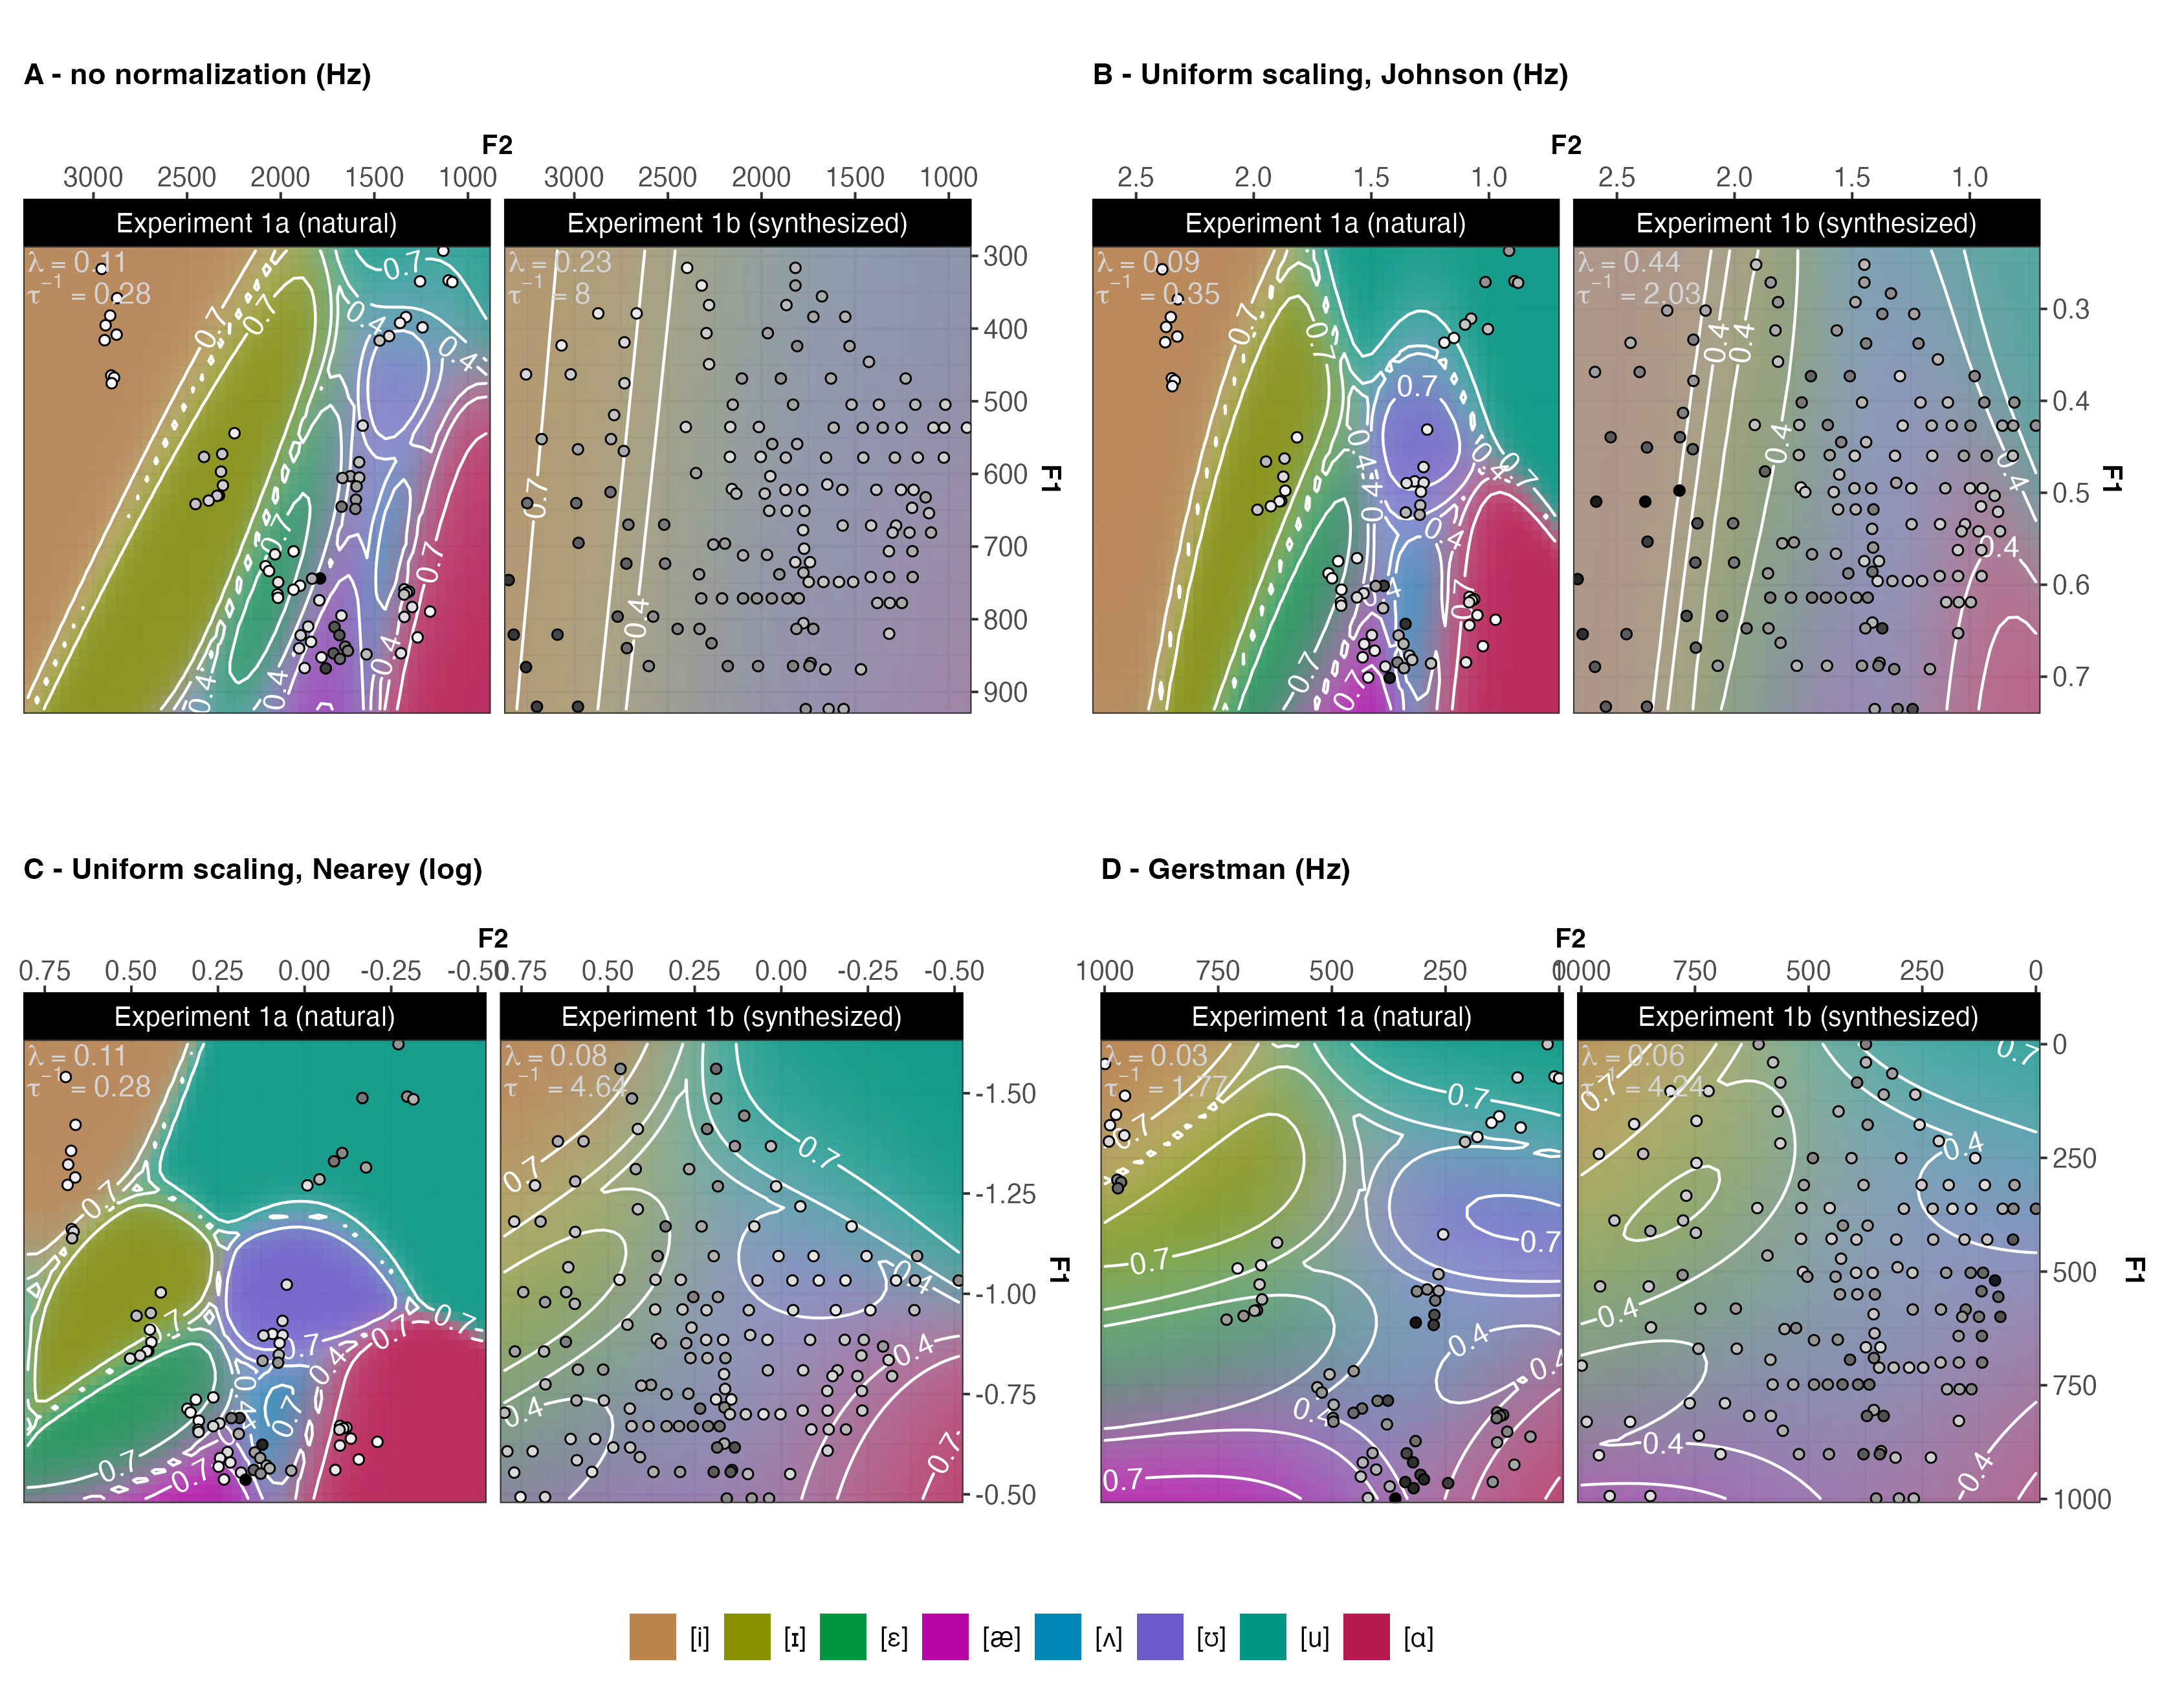
\includegraphics[width=0.8\linewidth]{../../figures/p.prediction-landscapes-study1} 

}

\caption{Predicted categorization functions over the F1-F2 space under \DIFdelbeginFL \DIFdelFL{four }\DIFdelendFL \DIFaddbeginFL \DIFaddFL{three }\DIFaddendFL different normalization accounts. For each account, we show the predicted posterior probabilities of all eight vowels obtained by averaging over the maximum likelihood parameterizations (of \(\lambda\) and \(\tau^{-1}\)) for the five training sets (shown at top of each panel). \DIFdelbeginFL \textbf{\DIFdelFL{Top:}} %DIFAUXCMD
\DIFdelendFL \DIFaddbeginFL \textbf{\DIFaddFL{Panel A:}} \DIFaddendFL absence of normalization shown for reference. \DIFdelbeginFL \textbf{\DIFdelFL{2nd row:}} %DIFAUXCMD
\DIFdelendFL \DIFaddbeginFL \textbf{\DIFaddFL{Panel B:}} \DIFaddendFL the best-fitting account for Experiment 1a. \DIFdelbeginFL \textbf{\DIFdelFL{3rd row:}} %DIFAUXCMD
\DIFdelendFL \DIFaddbeginFL \textbf{\DIFaddFL{Panel C:}} \DIFaddendFL the best-fitting account for Experiment 1b\DIFdelbeginFL \DIFdelFL{(and second best for Experiment 1a)}\DIFdelendFL . \DIFdelbeginFL \textbf{\DIFdelFL{Bottom:}} %DIFAUXCMD
\DIFdelFL{the second best-fitting account in Experiment 1b. }\DIFdelendFL Contours indicate the highest posterior probability of any vowel. Points indicate location of test stimuli. The increasing \DIFdelbeginFL \DIFdelFL{opacity }\DIFdelendFL \DIFaddbeginFL \DIFaddFL{brightness }\DIFaddendFL of points indicates a \DIFdelbeginFL \DIFdelFL{worse fit by }\DIFdelendFL \DIFaddbeginFL \DIFaddFL{better match between }\DIFaddendFL the account\DIFaddbeginFL \DIFaddFL{'s prediction and listeners' responses }\DIFaddendFL (\DIFaddbeginFL \DIFaddFL{higher log-likelihood; }\DIFaddendFL see text for detail).}\label{fig:prediction-landscapes-optim-io}
\end{figure}

Second, the best-fitting parameters (shown at the top of each panel) were relatively comparable across accounts but differed more substantially across experiments. Specifically, the best-fitting estimates of lapse rates \(\lambda\) were generally comparable across the two experiments (with the exception of Nordström \& Lindblom and Johnson normalization, which exhibited substantially higher lapse rates in Experiment 1b; SI \ref{sec:SI-param-est}). This suggests that participants in both experiments were about equally likely to pay attention to the stimulus. The best-fitting noise ratios \(\tau^{-1}\), however, differed substantially across experiments, and were \DIFdelbegin \DIFdel{9 }\DIFdelend \DIFaddbegin \DIFadd{10 }\DIFaddend times larger for Experiment 1b (mean \(\tau^{-1}\) = \DIFdelbegin \DIFdel{4.74}\DIFdelend \DIFaddbegin \DIFadd{4.32}\DIFaddend , SD = \DIFdelbegin \DIFdel{2.57 }\DIFdelend \DIFaddbegin \DIFadd{2.52 }\DIFaddend across normalization accounts) than for Experiment 1a (mean \(\tau^{-1}\) = \DIFdelbegin \DIFdel{0.52}\DIFdelend \DIFaddbegin \DIFadd{0.42}\DIFaddend , SD = \DIFdelbegin \DIFdel{0.49}\DIFdelend \DIFaddbegin \DIFadd{0.46}\DIFaddend ). This difference most likely reflects the fact that the synthesized stimuli in Experiment 1b left listeners with substantially more uncertainty about the intended category, as discussed during the description of the experiments.

Since noise is assumed to be independent of category variability \citep[see also][]{feldman2009, kronrod2016}, differences in noise ratios can substantially change the categorization function. This is particularly evident for the accounts that had more variable performance across the two experiments. For example, \DIFdelbegin \DIFdel{both Johnson (third row) and Lobanov normalization (fourth row}\DIFdelend \DIFaddbegin \DIFadd{Johnson normalization (Panel B}\DIFaddend ) resulted in very different best-fitting categorization functions for Experiments 1a and 1b.

Third and finally, Figure \ref{fig:prediction-landscapes-optim-io} also shows how well accounts fit listeners' responses for each test stimulus (opaqueness of the \DIFdelbegin \DIFdel{black }\DIFdelend points). This begins to explain \emph{why} some accounts fit listeners' responses in Experiment 1b less well. For example, the Johnson normalization account (\DIFdelbegin \DIFdel{third row}\DIFdelend \DIFaddbegin \DIFadd{Panel B}\DIFaddend ) predicts the responses to the test stimuli in Experiment 1a well, but fails to predict the responses to the test stimuli in Experiment 1b. This drop in performance seems to be primarily driven by stimuli that are unlikely to be articulated by the same talker (lower left, cf.~dashed line in Figure \ref{fig:human-performance}). This might suggest that this account was over-engineered to explain naturally occurring productions---the type of data, it was originally tested on \citep{johnson2020}. A plausible account of normalization, however, should be able to explain human perception to any type of stimulus, including synthesized stimuli. The SI (\ref{sec:SI-by-item}) presents more detailed by-item comparisons of normalization accounts that might be of interest to some readers.

\section{General discussion}\label{sec:G-D}

Research on vowel normalization has an influential history. Cognitive scientists have long aimed to understand the organization of frequency information in the human brain \citep{stevens-volkmann1940, siegel1965}, and how it helps listeners overcome cross-talker variability in the formant-to-vowel mapping \citep[e.g.,][]{joos1948, fant1975, nordstrom-lindblom1975}. Auditory processes that normalize speech inputs for differences in vocal tract physiology are now recognized to be an integral part of speech perception \citep{mcmurray-jongman2011, johnson-sjerps2021, xie2023}. Here, we set out to investigate what types of computations are implicated in the normalization of the frequency information that plays a critical role in the recognition of vowels.

Our results support three theoretical insights. First, human speech perception draws on more than psycho-acoustic transformations or intrinsic information, in line with previous research on normalization \citep{nearey1989, ladefoged-broadbent1957, adank2004}. Rather, formant normalization seems to involve the estimation and storing of talker-specific formant properties. Second, computationally simple uniform scaling accounts provide the best fit to listeners' responses, suggesting comparatively parsimonious maintenance of talker-specific properties. This replicates and extends previous findings that uniform scaling or similarly simple corrections for vocal tract size provide a better explanation for human perception than more complex extrinsic accounts \citep{barreda2021, richter2017}. It is impossible to rule out more complex approaches to perceptual normalization given the large number of possible alternatives. However, given that uniform scaling provides a parsimonious explanation for human formant normalization, and the current absence of empirical evidence for more complex computations, we submit that researchers ought to adapt uniform scaling as \DIFdelbegin \DIFdel{our }\DIFdelend \DIFaddbegin \DIFadd{the }\DIFaddend working hypothesis. Third, the psycho-acoustic representation assumed by different normalization accounts matter, as indicated by the comparison of otherwise computationally similar accounts (e.g.~Nearey's vs.~Johnson's uniform scaling).

\DIFdelbegin \DIFdel{These }\DIFdelend \DIFaddbegin \DIFadd{The }\DIFaddend results contribute to a still comparatively small body of work that has evaluated competing normalization accounts against listeners' perception, whereas most previous work evaluates accounts against intended productions. Complementing previous work, we took a broad-coverage approach: the present study compared 20 of the most influential normalization accounts against listeners' perception of \emph{hVd} words with \DIFdelbegin \DIFdel{all }\DIFdelend eight US English monophthongs in both natural and synthesized speech. This contrasts with previous work, which has typically focused on subsets of the vowel system, either using natural \emph{or} synthesized speech, and considering a much smaller subset of accounts (typically 2-3 at a time). By considering a wider range of accounts, a wider range of formant values and vowel categories, and multiple types of speech, we aimed to contribute to a more comprehensive evaluation of competing accounts.

Next, we discuss the theoretical consequences of these findings for research beyond formant normalization. Following that, we discuss limitations of the present work, and how future research might overcome them.

\subsection{Consequences for theories of speech perception and beyond}\label{consequences-for-theories-of-speech-perception-and-beyond}

Understanding the perceptual space in which the human brain represents vowel categories---i.e., the normalized formant space---has obvious consequences for research on speech perception. To illustrate how far reaching these consequences can be, we discuss a few examples. For instance, research on \emph{categorical perception} has found that vowels seem to be perceived less categorically than some types of consonants. Recent work has offered an elegant explanation for this finding: the perception of formants---relevant to the recognition of vowels---might be more noisy than the perception of the acoustic cues that are critical to the recognition of \DIFdelbegin \DIFdel{less }\DIFdelend \DIFaddbegin \DIFadd{more }\DIFaddend categorically perceived consonants \citep{kronrod2016}. This is a parsimonious explanation, potentially preempting the need for separate explanations for the perception of different types of phonemic contrasts. Kronrod and colleagues based their argument on estimates they obtained for the relative ratio of meaningful category variability to perceptual noise (\(\tau\), the inverse of our noise ratios, \(\tau^-1\)). Critically, this ratio depends both on (i) the perceptual space in which formants are assumed to be represented (Kronrod at al\DIFaddbegin \DIFadd{.~}\DIFaddend used Mel-transformed \DIFdelbegin \DIFdel{formants}\DIFdelend \DIFaddbegin \DIFadd{formant frequencies}\DIFaddend ), and on (ii) whether the meaningful category variability is calculated prior to, or following, normalization (Kronrod et al\DIFaddbegin \DIFadd{.~}\DIFaddend assumed the former, which increases estimates of category variability). Our point here is not to cast doubt on the results of \citet{kronrod2016} ---the fact that the best-fitting noise ratios in our study were relatively similar across accounts (while varying across experiments) suggests that the result of Kronrod and colleagues are likely to hold even under different assumptions about (i) and (ii)---but rather to highlight how research on the perception and recognition of vowels depends on assumptions about formant normalization. For example, similar points could be raised about experiments on statistical learning that manipulate formant or other frequency statistics \citep[e.g.,][]{chladkova2017, colby2018, xie2021, wade2007}. Such experiments, too, need to make assumptions about the space in which formants are represented. If these assumptions are incorrect, this can affect whether the experimental manipulations have the intended effects, increasing the chance of null effects or misinterpretation of observed effects.

Understanding the perceptual space in which the human brain represents vowel categories also has consequences for research beyond speech perception, perhaps more so than is sometimes recognized. For instance, in sociolinguistics and related fields, Lobanov remains the norm for representing vowels due to its efficiency in removing cross-talker variability \citep[for review, see][]{adank2004, barreda2021}. However, as shown in the present study, removing cross-talker variability is not the same as representing vowels in the perceptual space that listeners actually employ. Here, we do \emph{not} find Lobanov to describe human perception particularly well. On the contrary, we find no support for the hypothesis that human speech perception employs these more complex computations that have been found to perform best at reducing category variability. This should worry sociolinguists. In order to understand how listeners infer a talker's background or social identity, it is important to understand the perceptual space in which inferences are actually rooted. Critically, the representations resulting from formant normalization presumably form an important part of the information that listeners use to draw social and linguistic inferences. It should thus be obvious that the use of normalization accounts that do not actually correspond to human perception can both mask real markers of social identity, and \DIFdelbegin \DIFdel{hallucinate }\DIFdelend \DIFaddbegin \DIFadd{`hallucinate' }\DIFaddend markers that are not actually present. For example, in order to determine how a talker's social identity influences their vowel realizations, it is important to discount \emph{all and only} effects that listeners \DIFdelbegin \DIFdel{' }\DIFdelend will attribute to physiology, rather than social identity \citep{disner1980, hindle1978}.

Similar concerns apply to dialectology, research on language change, second language acquisition research, etc. For example, the perceptual space in which vowels are represented is critical to well-formed tests of hypotheses about the factors shaping the organization of vowel inventories across languages of the world \citep{lindblom1986, stevens1972, stevens1989}. It is essential in testing hypotheses about the extent to which the cross-linguistic realization of those systems is affected by perceptual processes \DIFdelbegin %DIFDELCMD < \citep{flemming2010, steriade2001}%%%
\DIFdelend \DIFaddbegin \citep{flemming2010, steriade2008}\DIFaddend , or by preferences for communicatively efficient linguistic systems \citep[e.g.,][]{hall2018, lindblom1990, moulin2015}. Similarly, tests of the hypothesis that vowel \emph{articulation} during natural interactions is shaped by communicative efficiency do in obvious ways depend on assumptions about the perceptual space in which talkers---by hypothesis---aim to reduce perceptual confusion \citep[cf.][]{buz-jaeger2016, gahl2012, scarborough2010, wedel2018}. The same applies to any other line of research that aims to understand the perceptual consequences of formant variation across talkers, including research on infant- or child-directed speech \citep{eaves2016, kuhl1997}, and research on whether non-native talkers are inherently more variable than native talkers \citep{smith2019, vaughn2019, xie-jaeger2020}. In short, the perceptual space in which vowels are represented is a critical component of understanding the structure of vowel systems, the factors that shape them, and the ways in which they are used in natural language.

\subsection{Limitations and future directions}\label{limitations-and-future-directions}

\DIFdelbegin \DIFdel{The present work shares a few limitations with previous work. Here we focus on limitations that follow from the assumptions }\DIFdelend \DIFaddbegin \DIFadd{As mentioned in the introduction, we take it as relatively uncontroversial }\emph{\DIFadd{that}} \DIFadd{normalization is part of human speech perception. Independent of any benefits that such normalization conveys for speech perception, its existence is supported by evidence from cross-species comparisons and neuro-physiological studies }\citep[for review, see][]{barreda2020}\DIFadd{. There are, however, important questions as to how decisions }\DIFaddend we made in \DIFdelbegin \DIFdel{our computational framework.
While theories and hypotheses often contain substantial vagueness, }\emph{\DIFdel{quantitative tests}} %DIFAUXCMD
\DIFdel{of those }\DIFdelend \DIFaddbegin \DIFadd{comparing normalization accounts against each other might have affected their fit against listeners' responses.
}

\DIFadd{For instance, we followed previous work in focusing on formants, and specifically estimates of the formants in the }\emph{\DIFadd{center}} \DIFadd{of the vowel. There is, however, ample evidence that formant dynamics throughout the vowel can strongly affect perception }\citetext{\citealp[\citet{hillenbrand-nearey1999}]{assmann-katz2005}; \citealp{nearey-assmann1986}}\DIFadd{. In addition, there are proposals that entirely give up the assumption that formants are the primary cues to vowel identity }\citep[e.g., whole-spectrum accounts,][]{hillenbrand2006}\DIFadd{. While these proposals might provide a more informative representation of vowels, we consider it unlikely that they would entirely remove the problem of cross-talker variability. For instance, }\citet{richter2017} \DIFadd{still found benefits of normalization even when the entire frequency spectrum throughout vowels was considered (in the form of Mel-Frequency Cepstral Coefficients and their derivatives). For the present work, auxiliary analyses in the SI (\ref{sec:SI-F1F3}) replicated our core findings when F3 was included in the model. Still, it remains unclear whether the inclusion of additional cues, such as VISC, or additional formant dynamics, would alter the results of the present study.
}

\DIFadd{As is the case of any computational work, the present study committed to a number of assumptions that are not critical, but were necessary in order to deliver clear quantitative predictions. Quantitative tests of }\DIFaddend theories---as we have done here---require assumptions about \emph{every} aspect of the model. Here, this included all the steps necessary to link properties of the stimuli to listeners' responses. For this purpose, we adopted the ASP framework \citep{xie2023}, and visualized the graphical model that links stimuli (\(x\)) to responses (\(r\)) in Figure \ref{fig:model-perceptual-decision-making}.

Many of the assumptions we made should be \DIFdelbegin \DIFdel{quite }\DIFdelend \DIFaddbegin \DIFadd{relatively }\DIFaddend uncontroversial---e.g., the decision to include both external (environmental) and internal (perceptual) noise in our model. While these noise sources are often ignored in modeling human behavior, it is uncontroversial that they exist. Other assumptions we made were introduced as simplifying assumptions for the sake of feasibility---e.g., we expressed the effect of both types of noise through a single parameter that related the average within-category variability of formants to noise variability in the transformed and normalized formant space. In reality, however, environment noise can have effects that are independent of internal noise, and internal noise likely affects information processing at multiple (or all) of the steps shown in Figure \ref{fig:model-perceptual-decision-making}. Such simplifying assumptions are both inevitable, and not necessarily problematic: as long as they do not introduce systematic bias to the evaluation of normalization accounts, they should not limit the generalizability of our results.

Some of our assumptions, however, might be more controversial. For example, we assumed that category representations can be expressed as multivariate Gaussian distributions in the formant space. This assumption, too, is a simplifying assumption---it simplified the computation of likelihoods---rather than a critical feature of the ASP framework we employed. While human category representations are unlikely to be Gaussians, the alternative, e.g., exemplar representations, would come with its own downsides, such as increased sensitivity to the limited size of phonetic databases and substantial increases in computation time (exemplar representations afford researchers with much larger degrees of freedom). For researchers curious how this and other assumptions we made affect our results, our data and code are shared on OSF.
\DIFdelbegin \DIFdel{This includes the R markdown document that generates this PDF, making it comparatively easy to revisit any of our assumptions to then regenerate the entire study with a click of a button in RStudio.
}\DIFdelend 

Like previous work, we further assumed that all listeners in our experiments use the same underlying vowel representations---the same dialect template(s). However, as already discussed, it is rather likely that not all of our listeners employed the same dialect template(s). An additional analysis reported in the SI (\ref{sec:SI-dialect-subset}) thus compared normalization accounts against only the subset of listeners who employed the dialect template used by the majority of participants (see lower-left of Figure \ref{fig:human-confusion}B). This left only \DIFdelbegin \DIFdel{11 }\DIFdelend \DIFaddbegin \DIFadd{20 }\DIFaddend participants for Experiment 1a (\DIFdelbegin \DIFdel{61.1}\DIFdelend \DIFaddbegin \DIFadd{71.4}\DIFaddend \%) and \DIFdelbegin \DIFdel{14 }\DIFdelend \DIFaddbegin \DIFadd{23 }\DIFaddend for Experiment 1b (\DIFdelbegin \DIFdel{77.8}\DIFdelend \DIFaddbegin \DIFadd{82.1}\DIFaddend \%), substantially reducing statistical power. Replicating the main analysis, uniform scaling accounts again fit listeners' behavior well across both experiments. The best-performing \DIFdelbegin \DIFdel{accounts }\DIFdelend \DIFaddbegin \DIFadd{account for Experiment 1a }\DIFaddend did, however, differ from the \DIFdelbegin \DIFdel{ones }\DIFdelend \DIFaddbegin \DIFadd{one }\DIFaddend obtained for the superset of data (\DIFaddbegin \DIFadd{the intrinsic Syrdal \& Gopal achieved the best fit to listeners' responses in Experiment 1a for the shared dialect subset; }\DIFaddend see SI, \ref{sec:SI-dialect-subset}).

A related assumption was introduced by the use of a phonetic database to approximate listeners' vowel representations. This deviates from most previous evaluations of normalization accounts \citetext{\citealp{mcmurray-jongman2011}; \citealp{barreda2021}; \citealp[but see][]{richter2017}}, and reflects our commitment to a strong assumption made by most theories of speech perception: that listeners' representations reflect the formant statistics previously experienced speech input. By using a phonetic database to estimate listeners' representations, we \emph{substantially} reduced the degrees of freedom in the evaluation of normalization accounts, reducing the chance of over-fitting to the data from our experiments. Our approach does, however, also introduce two new assumptions.

First, our approach assumes that the mixture of dialect template(s) used by talkers in the database sufficiently closely approximates those of the listeners in our experiments. Some validation for this assumption comes from the additional analysis reported in the preceding paragraph: when we subset listeners to only those who used the majority dialect template, this improved the fit of all normalization accounts---as expected, if the category representations we trained on the phonetic database primarily reflect those listeners' representations (see SI, \ref{sec:SI-dialect-subset}). Future work could further address this assumption in a number of ways. On the one hand, dialect analyses like the ones we presented for our listeners (in Figure \ref{fig:human-confusion}B) could compare listeners' templates against the templates used by talkers in the database. Alternatively or additionally, researchers could see whether our results replicate if ideal observers are instead trained on other databases that have been hypothesized to reflect a `typical' L1 listeners' experience with US English. \DIFaddbegin \DIFadd{Finally, it might be possible in future work to use larger databases of vowel recordings to train separate ideal observers for all major dialects of US English, and to try to }\emph{\DIFadd{estimate}} \DIFadd{for each listener which mixture of dialects their responses are based on.
}\DIFaddend 

Second, we made the simplifying assumption that listeners' category representation---or at least the representations listeners' drew on during the experiment---are talker-\emph{independent} (we trained a single set of multivariate Gaussian categories, rather than, e.g., hierarchically organized set of multiple dialect templates). While this assumption is routinely made in research on normalization and beyond, it might well be wrong \citep[see e.g.,][]{xie2021}.

Finally, the evaluation of normalization accounts in the present \DIFdelbegin \DIFdel{work }\DIFdelend \DIFaddbegin \DIFadd{study }\DIFaddend shares with all previous work \citep[e.g.,][]{apfelbaum-mcmurray2015, cole2010, mcmurray-jongman2011, barreda2021, nearey1989, richter2017} another simplifying assumption that is clearly wrong: the assumption that listeners \emph{know} the talker-specific formant properties required for normalization. Specifically, we normalized the input for each ideal observer using the maximum likelihood estimates of the normalization parameters \DIFaddbegin \DIFadd{over all stimuli }\DIFaddend for the respective experiment. For example, for the evaluation of the ideal observer trained on Lobanov normalized formants against listeners' responses in Experiment 1a, we used the formant means and standard deviations of the stimuli used in Experiment 1a to normalize F1 and F2. While this follows previous work, it constitutes a problematic assumption for the evaluation of extrinsic normalization accounts. For \DIFdelbegin \DIFdel{these }\DIFdelend \DIFaddbegin \DIFadd{extrinsic }\DIFaddend accounts, the approach adopted \DIFdelbegin \DIFdel{essentially assumes }\DIFdelend \DIFaddbegin \DIFadd{here would seem to entail }\DIFaddend the ability to predict the future: even on the first trial of the experiment, the input to the ideal observers were formants that were normalized based on the \DIFdelbegin \DIFdel{maximum likelihood estimate of the normalization parameters given }\DIFdelend \DIFaddbegin \DIFadd{normalization parameters estimated over }\DIFaddend the acoustic properties of \emph{all} stimuli. Listeners instead need to \emph{incrementally infer} talker-specific properties from the speech input \DIFdelbegin %DIFDELCMD < \citep{nearey-assmann2007, xie2023}%%%
\DIFdel{. The development and testing of incremental variants of formant normalization strikes us an important avenue for future research. }\DIFdelend \DIFaddbegin \citep{barreda-jaeger2025, nearey-assmann2007, xie2023}\DIFadd{. An important avenue for future research is thus the development and evaluation of incremental normalization accounts.
}\DIFaddend 

\DIFaddbegin \DIFadd{The present data only allow an initial, rather tentative, look at this question. For example, for Experiment 1a, for which each trial had a known correct answer (the vowel intended by the talker), we can assess whether participants' recognition accuracy improved across trials, as would be expected if listeners need to incrementally infer the talker-specific normalization parameters. Figure \ref{fig:trial-accuracies}A suggests that this was indeed the case: the non-parametric listeners' average recognition accuracy improved over the course of the experiment from about 65\% to 88\%, with most of the improvements occurring during the first ten trials. To address potential confounds due to differences in the distribution of stimuli across trials, we used a generalized additive mixed-effect model to predict listeners' accuracy from log-transformed trial order while accounting for random by-participant and by-item intercepts and slopes for the log-transformed trial order (blue lines). Still, this result should be interpreted with caution, as Experiment 1a was not designed to reliably address questions about incremental changes across the experiment.
}

\DIFadd{Figure \ref{fig:trial-accuracies}B shows how the fit of the best-fitting normalization model changes across trials. We used a generalized additive mixed-effect model to predict the log-likelihood of listeners' responses from log-transformed trial order while accounting for random by-participant and by-item intercepts and slopes for the log-transformed trial order (blue lines). Given that our evaluation of normalization accounts assumed that the normalization parameters were already known on the first trial of the experiment, we would expect that the likelihood of listeners' responses under a normalization model would improve the more input listeners have received (i.e., as the simplifying assumptions of our evaluation become increasingly more plausible). For Experiment 1a, this indeed appears to be the case. However, no clear evidence for such incremental improvements in the fit of the normalization model is observed for Experiment 1b. In short, the present data does not support decisive conclusions about the extent to which normalization proceeds incrementally.
}



\begin{figure}[!ht]

{\centering \includegraphics[width=0.9\linewidth]{../../figures/knitted/trial-accuracies} 

}

\caption{\textbf{\DIFaddFL{Panel A}}\DIFaddFL{: Changes across trials in listeners' average accuracy in recognizing the vowel intended by the talker in Experiment 1a, averaged across items and participants (black line). Blue line shows a generalized additive mixed-effects model predicting accuracy from log-transformed trial order, with 95\% CIs. }\textbf{\DIFaddFL{Panel B}}\DIFaddFL{: Log-likelihood of listeners' responses under the best-fitting normalization account at each trial, averaged across items and participants (Johnson's uniform scaling for Experiment 1a and Nearey's uniform scaling for Experiment 1b). Blue lines show generalized additive mixed-effects models predicting log-likelihood from log-transformed trial order, with 95\% CIs.}}\label{fig:trial-accuracies}
\end{figure}

\DIFaddend \subsection{Concluding remarks}\label{concluding-remarks}

We set out to compare how well competing accounts of formant normalization explain listeners' perception of vowels. We developed a computational framework that makes it possible to compare a large number of different accounts against multiple data sets. The code we share on OSF makes it possible to `plug in' different accounts of vowel normalization, different phonetic databases, and different perception experiments. This, we hope, will substantially reduce the effort necessary to conduct similar evaluations on other datasets, dialects, and languages.

Comparing 20 of the most influential normalization accounts against L1 listeners' perception of US English monophthongs, we found that the normalization accounts that best describe listeners' perception share that they (1) learn and store talker-specific properties and (2) \DIFdelbegin \DIFdel{that they }\DIFdelend seem to be computationally very simple---taking advantage of the physics of sound generation to use as few as a single parameter to normalize inter-talker variability in vocal tract size. While the number of studies that have compared normalization accounts against \emph{listeners'} behavior remains surprisingly small, these two results confirm the findings from more targeted comparisons that were focused on 2-3 accounts at a time \citep{barreda2021, nearey1989, richter2017}. Overall then, we submit that it is time for research in speech perception and beyond to consider simple uniform scaling the most-likely candidate for human formant normalization.

\begin{acknowledgments}
Earlier versions of this work were presented at 2023 ASA meeting, ExLing 2022, at the Department of Computational Linguistics at the University of Zürich and at the Department of Swedish language and multilingualism at Stockholm University. We are grateful to \DIFdelbegin \DIFdel{OMITTED FOR REVIEW. }\DIFdelend \DIFaddbegin \DIFadd{Maryann Tan, Chigusa Kurumada, and Xin Xie for feedback on this work. We thank Travis Wade for clarifications on the synthesis procedure used in his study. We thank Leslie Li and Xin Xie for sharing their database of L1-US English *hVd* productions, and the JASA copy editing staff for help with the Latex formatting. This work was partially funded by grants to AP from Kungliga Vetenskapsakademien, Kungliga Vitterhetsakademien, and the Department of Swedish Language and Multilingualism at Stockholm University, as well as grants to TFJ by the Helge Ax:son Johnson foundation, the Stockholm University Board of Human Science (Funding for Strategic Investments), and the Stockholm University Faculty of Humanities’ Research School (Kvalitetssäkrande medel grant).
}\DIFaddend \end{acknowledgments}

\section*{Author Contributions}\label{author-contributions}
\addcontentsline{toc}{section}{Author Contributions}

AP designed the experiments and collected the data, with input from TFJ. TFJ programmed the experiments with input from AP. AP analyzed the experiments, with input from TFJ. AP and TFJ wrote the code to implement and fit the normalization models, with input from SB. AP developed the visualizations within input from SB and TFJ. AP wrote the first draft of the manuscript with edits by SB and TFJ.

\section*{Author Declarations}\label{author-declarations}
\addcontentsline{toc}{section}{Author Declarations}

\subsection*{Conflict of Interest}\label{conflict-of-interest}
\addcontentsline{toc}{subsection}{Conflict of Interest}

The authors \DIFdelbegin \DIFdel{declare that the research was conducted in the absence of any commercial or financial relationships that could be construed as a potential conflict of interest}\DIFdelend \DIFaddbegin \DIFadd{have no conflicts to disclose}\DIFaddend .

\subsection*{Ethics approval}\label{ethics-approval}
\addcontentsline{toc}{subsection}{Ethics approval}

This study was reviewed and approved Research Subjects Review Board (RSRB) of the University of Rochester (STUDY00000417) under the OHSP and UR policies, and in accordance with Federal regulation 45 CFR 46 under the university's Federal-wide Assurance (FWA00009386).

\newpage{}

\section{References}\label{sec:references}

\begingroup
\setlength{\parindent}{-0.5in}
\setlength{\leftskip}{0.5in}

\DIFaddbegin \nocite{balzano1982}
\DIFaddend \nocite{barreda-nearey2018}
\nocite{goldinger1996}
\nocite{hay2017}
\nocite{hay2019}
\nocite{johnson1999}
\nocite{kleinschmidt-jaeger2016}
\nocite{mcgowan2015}
\DIFaddbegin \nocite{shankweiler1978}
\DIFaddend \nocite{shannon1948}
\DIFaddbegin \nocite{strange-jenkins2012}
\DIFaddend \nocite{sumner2011}
\nocite{walker-hay2011}
\DIFaddbegin \nocite{zwicker1957}
\nocite{zwicker-terhardt1980}
\DIFaddend 

\endgroup

% -------------------------------------------------------------------------------------------------------------------
%   Appendix  (optional)

%\appendix
%\section{Appendix title}

%If only one appendix, please use
%\appendix*
%\section{Appendix title}


%=======================================================

%Use \bibliography{<name of your .bib file>}+
%to make your bibliography with BibTeX.

%=======================================================

\bibliography{latex-stuff/library.bib,latex-stuff/r-references.bib}


\end{document}
